%! Author = crist
%! Date = 25/10/2026

\spacing{1.3}
%----------------------------------------------------------------------------------------
%	UNIDAD 10: FUERZAS EN LOS FLUIDOS (4.º ESO)
%   Figuras: images/UD10/*.pdf (fuente HTML en images/UD10/html, SVG en images/UD10/svg)
%   Gráficas con pgfplots: estilo «grafica», definido al inicio de la UD7.
%   Unidades \atm y \mmHg: declaradas al inicio de la UD5.
%   Datos usados en toda la unidad: g = 9,8 m/s², ρ(agua) = 1000 kg/m³, ρ(agua de mar) = 1030 kg/m³,
%   1 atm = 760 mmHg = 1,013·10^5 Pa.
%----------------------------------------------------------------------------------------

% Mapa conceptual del tema (fuente en images/mapas_conceptuales/html/temas.js)
\begin{figure}[H]
    \centering
    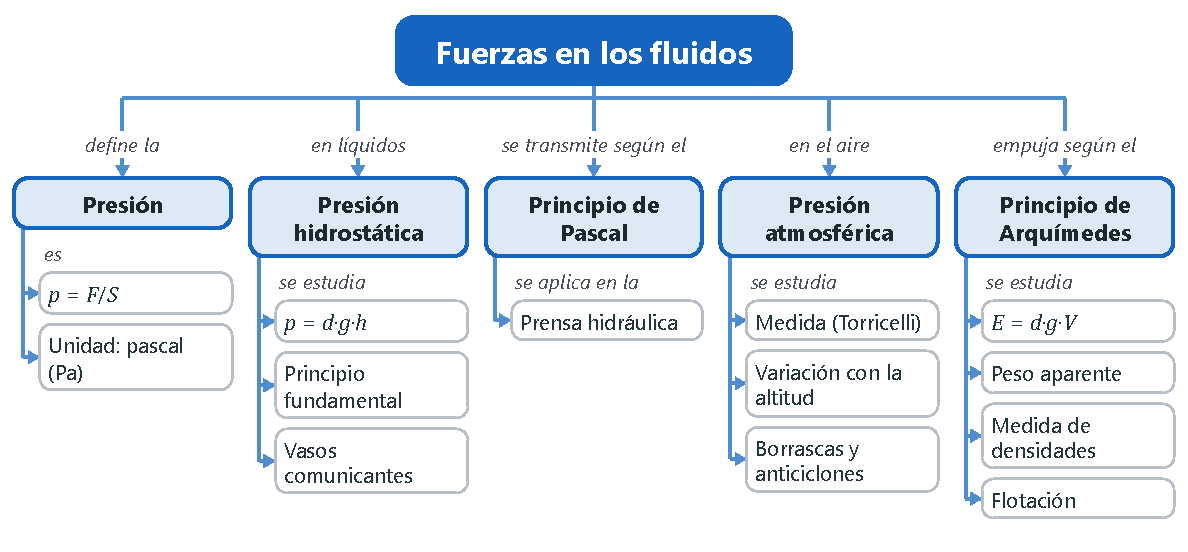
\includegraphics[width=\textwidth]{images/mapas_conceptuales/mapa_UD10}
\end{figure}

%========================================================================================
%\section*{Para empezar: la meteorología moderna}
%\addcontentsline{toc}{section}{Para empezar: la meteorología moderna}
%========================================================================================
%
%A comienzos del siglo \textsc{xx}, el noruego \textbf{Vilhelm Bjerknes} propuso tratar la predicción del tiempo como un problema de física: si se conoce con detalle el estado de la atmósfera en un momento dado (presión, temperatura, humedad, viento\ldots), las leyes de la física permiten calcular cómo va a evolucionar. Esa idea es la base de las predicciones actuales.
%
%Sin embargo, llevarla a la práctica no era fácil. Casi no había observaciones de las capas altas de la atmósfera, hasta que la aviación permitió tomar datos a gran altura. Además, los cálculos eran tan largos que el tiempo «pasaba» antes de terminarlos; el problema se resolvió con la llegada de los ordenadores. Desde el lanzamiento del primer satélite artificial, en 1957, la atmósfera también se observa desde el espacio.
%
%Una buena predicción no evita una tormenta, pero sí puede salvar vidas: avisar a tiempo permite preparar planes de emergencia ante inundaciones, temporales u olas de calor. Por eso la meteorología está relacionada con el \textbf{ODS 11} (\emph{Ciudades y comunidades sostenibles}), que busca reducir las muertes causadas por desastres naturales, y con el \textbf{ODS 13} (\emph{Acción por el clima}), que pide reforzar la capacidad de adaptación a los riesgos del clima.
%
%En esta unidad estudiaremos la \textbf{presión}, una magnitud imprescindible para entender los fluidos: por qué un buzo no puede bajar a cualquier profundidad, cómo funciona un gato hidráulico, qué mide un barómetro, qué significan las borrascas y los anticiclones de los mapas del tiempo y por qué flota un barco de acero.
%
%\begin{exercise}
%    ¿Qué idea de Bjerknes es la base de las predicciones meteorológicas actuales?
%    \begin{solu}
%        Tratar la predicción del tiempo como un \textcolor{red}{problema de física}: a partir del estado de la atmósfera en un instante (los «valores iniciales»), calcular con las leyes de la física cómo evolucionará.
%    \end{solu}
%\end{exercise}
%
%\begin{exercise}
%    ¿Qué dos dificultades había a comienzos del siglo \textsc{xx} para aplicar esa idea? ¿Cómo se resolvieron?
%    \begin{solu}
%        No había apenas \textcolor{red}{observaciones de las capas altas} de la atmósfera, lo que se resolvió con el desarrollo de la \textcolor{red}{aviación}; y los \textcolor{red}{cálculos eran muy largos}, lo que se resolvió con los \textcolor{red}{ordenadores}.
%    \end{solu}
%\end{exercise}
%
%\begin{exercise}
%    ¿Han sido útiles los satélites artificiales para la meteorología? Busca el nombre de algunos satélites meteorológicos y la altura a la que operan.
%    \begin{solu}
%        Sí, son \textcolor{red}{fundamentales}: observan continuamente grandes zonas de la atmósfera. Por ejemplo, los \textcolor{red}{Meteosat} europeos son geoestacionarios (a unos \qty{36000}{\km} de altura); otros, como los MetOp, son de órbita polar (a unos \qty{800}{\km}).
%    \end{solu}
%\end{exercise}
%
%\begin{exercise}
%    ¿Cómo puede ayudar la predicción meteorológica a reducir los daños de los desastres naturales? ¿Qué relación tiene con los ODS 11 y 13? Debatidlo en clase.
%    \begin{solu}
%        Respuesta libre. Prever con antelación una situación de emergencia permite \textcolor{red}{avisar a la población y preparar recursos}, lo que evita pérdidas de vidas y reduce daños en las ciudades (ODS 11) y mejora la adaptación a los riesgos del clima (ODS 13).
%    \end{solu}
%\end{exercise}

%========================================================================================
\section[Fuerza y superficie: la presión]{¿Existe una relación entre la intensidad de una fuerza y la superficie sobre la que actúa? La presión}
%========================================================================================

Si dejamos caer un prisma sobre una capa de plastilina o de arcilla, siempre desde la misma altura, la huella es más profunda cuanto \textbf{menor} es la cara sobre la que cae (figura~\ref{fig:presion_superficie}). Y si usamos prismas más pesados, las huellas son más profundas. El efecto de una fuerza depende, por tanto, de su intensidad y del tamaño de la superficie sobre la que actúa.

\begin{definition}[Presión]
    La \textbf{presión}, \(p\), es la fuerza que actúa perpendicularmente sobre cada unidad de superficie:
    \[ p = \frac{F}{S} \]
    donde \(F\) es el módulo de la fuerza y \(S\) el área de la superficie. En el SI se mide en \textbf{newton por metro cuadrado} (\unit{\newton\per\square\m}), unidad que se llama \textbf{pascal} (\unit{\pascal}): \(\qty{1}{\pascal} = \qty{1}{\newton\per\square\m}\).
\end{definition}

La presión es una \textbf{magnitud escalar}: en un punto tiene el mismo valor en todas las direcciones. Su ecuación de dimensiones es \([p] = \mathrm{M \cdot L^{-1} \cdot T^{-2}}\).

Con una superficie pequeña se consiguen presiones muy grandes aplicando fuerzas pequeñas. Por eso los cuchillos afilados cortan mejor que los romos y las puntas finas de los clavos, chinchetas y agujas penetran con facilidad. Al revés, para \emph{repartir} una fuerza se aumenta la superficie: las raquetas de nieve, los esquís o las orugas de un tractor evitan que se hundan en el terreno.

\begin{figure}[H]
    \centering
    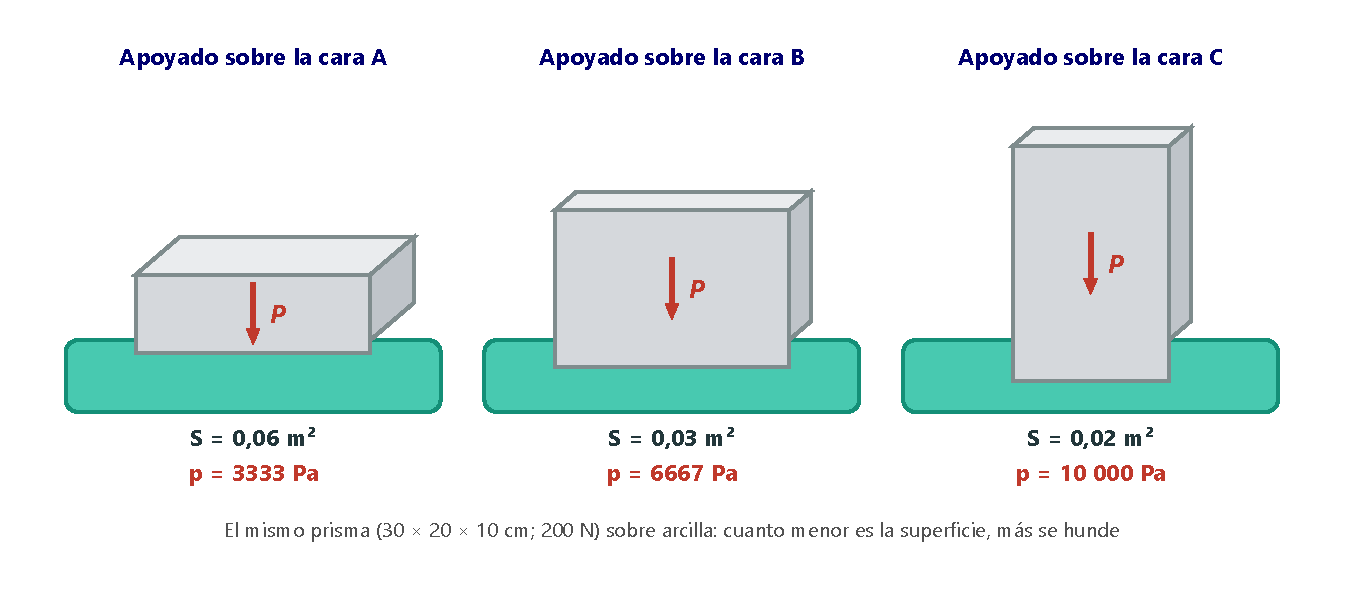
\includegraphics[width=\textwidth]{images/UD10/presion_superficie}
    \caption{Un mismo prisma ejerce más presión cuanto menor es la cara sobre la que se apoya.}
    \label{fig:presion_superficie}
\end{figure}

\begin{example}
    Un prisma rectangular de \(30 \times 20 \times 10\)~\unit{\cm} pesa \qty{200}{\newton}. Calcula la presión que ejerce sobre el suelo cuando se apoya sobre cada una de sus caras.

    Cara A (\(30 \times 20\)): \(S_A = \num{0.30} \cdot \num{0.20} = \qty{0.06}{\square\m}\); \quad \(p_A = \dfrac{200}{\num{0.06}} = \textcolor{red}{\qty{3333}{\pascal}}\).

    Cara B (\(30 \times 10\)): \(S_B = \num{0.30} \cdot \num{0.10} = \qty{0.03}{\square\m}\); \quad \(p_B = \dfrac{200}{\num{0.03}} = \textcolor{red}{\qty{6667}{\pascal}}\).

    Cara C (\(20 \times 10\)): \(S_C = \num{0.20} \cdot \num{0.10} = \qty{0.02}{\square\m}\); \quad \(p_C = \dfrac{200}{\num{0.02}} = \textcolor{red}{\qty{10000}{\pascal}}\).

    Al disminuir la superficie, aumenta la presión.
\end{example}

\begin{exercise}
    Escribe la ecuación de dimensiones de la presión a partir de su definición.
    \begin{solu}
        \([p] = \dfrac{[F]}{[S]} = \dfrac{\mathrm{M \cdot L \cdot T^{-2}}}{\mathrm{L^2}} = \textcolor{red}{\mathrm{M \cdot L^{-1} \cdot T^{-2}}}\).
    \end{solu}
\end{exercise}

\begin{exercise}
    Haz una lista de objetos que tengan filo o punta y explica para qué sirven.
    \begin{solu}
        Respuesta libre: cuchillos, tijeras, abrecartas, chinchetas, agujas, alfileres, clavos\ldots{} Todos sirven para cortar, clavar o penetrar en una superficie, porque su filo o su punta tienen una \textcolor{red}{superficie muy pequeña} y permiten ejercer \textcolor{red}{presiones muy elevadas} con fuerzas pequeñas.
    \end{solu}
\end{exercise}

\begin{exercise}
    Golpeamos con la misma fuerza dos clavos iguales: uno por la cabeza y otro por la punta (con la cabeza apoyada en la madera). ¿Cuál penetrará más fácilmente? ¿Por qué?
    \begin{solu}
        El que se golpea por la \textcolor{red}{cabeza}, porque la fuerza actúa sobre la madera a través de la punta, que tiene una superficie mucho menor: la \textcolor{red}{presión es mayor}.
    \end{solu}
\end{exercise}

\begin{exercise}
    Un prisma rectangular mide \(30 \times 20 \times 40\)~\unit{\cm} y pesa \qty{100}{\newton}. Calcula la presión que ejerce sobre una capa de arcilla al apoyarlo sobre cada una de sus caras.
    \begin{solu}
        Cara de \(30 \times 20\): \(p = \dfrac{100}{\num{0.3} \cdot \num{0.2}} = \textcolor{red}{\qty{1667}{\pascal}}\).
        Cara de \(30 \times 40\): \(p = \dfrac{100}{\num{0.3} \cdot \num{0.4}} = \textcolor{red}{\qty{833}{\pascal}}\).
        Cara de \(20 \times 40\): \(p = \dfrac{100}{\num{0.2} \cdot \num{0.4}} = \textcolor{red}{\qty{1250}{\pascal}}\).
    \end{solu}
\end{exercise}

\begin{exercise}
    Calcula la presión que ejerce una fuerza de \qty{100}{\newton} si se aplica sobre:
    \begin{enumerate}[label=\alph*)]
        \item Una superficie circular de \qty{20}{\cm} de radio.
        \item Una superficie cuadrada de \qty{20}{\cm} de lado.
    \end{enumerate}
    \begin{solu}
        a) \(S = \pi \cdot \num{0.20}^2 = \qty{0.126}{\square\m}\); \(p = \dfrac{100}{\num{0.126}} = \textcolor{red}{\qty{796}{\pascal}}\).
        b) \(S = \num{0.20}^2 = \qty{0.04}{\square\m}\); \(p = \dfrac{100}{\num{0.04}} = \textcolor{red}{\qty{2500}{\pascal}}\).
    \end{solu}
\end{exercise}

\begin{exercise}
    Un esquiador que pesa \qty{800}{\newton} se desliza con unos esquís de \qty{1200}{\square\cm} de superficie cada uno. ¿Qué presión ejerce sobre la nieve? ¿Y si estuviera de pie con unas botas de \qty{300}{\square\cm} cada una?
    \begin{solu}
        Con esquís: \(S = 2 \cdot \qty{0.12}{\square\m} = \qty{0.24}{\square\m}\); \(p = \dfrac{800}{\num{0.24}} = \textcolor{red}{\qty{3333}{\pascal}}\).
        Con botas: \(S = 2 \cdot \qty{0.03}{\square\m} = \qty{0.06}{\square\m}\); \(p = \dfrac{800}{\num{0.06}} = \textcolor{red}{\qty{13333}{\pascal}}\), cuatro veces más: por eso con botas se hunde en la nieve.
    \end{solu}
\end{exercise}

\subsection*{Actividades de consolidación: la presión}

\begin{exercise}
    Responde verdadero o falso y justifica tu respuesta:
    \begin{enumerate}[label=\alph*)]
        \item Un cuchillo afilado corta mejor que uno romo porque en su filo la presión es menor.
        \item El efecto de una fuerza depende del tamaño de la superficie sobre la que actúa.
        \item Para una misma fuerza, la presión es mayor cuanto mayor es la superficie sobre la que actúa.
    \end{enumerate}
    \begin{solu}
        a) \textcolor{red}{Falso}: corta mejor porque en su filo la presión es \emph{mayor}. b) \textcolor{red}{Verdadero}. c) \textcolor{red}{Falso}: la presión es mayor cuanto \emph{menor} es la superficie.
    \end{solu}
\end{exercise}

\begin{exercise}
    Una aguja de coser de \qty{e-6}{\square\m} de sección ejerce una presión de \qty{4e7}{\pascal} sobre la tela. ¿Con qué fuerza se ha empujado la aguja? ¿Qué presión ejercería si se duplicara la fuerza?
    \begin{solu}
        \(F = p \cdot S = \num{4e7} \cdot \num{e-6} = \textcolor{red}{\qty{40}{\newton}}\). Si la fuerza se duplica, también lo hace la presión: \(p = \textcolor{red}{\qty{8e7}{\pascal}}\).
    \end{solu}
\end{exercise}

\begin{exercise}
    La punta de un clavo tiene \qty{0.1}{\square\mm} de superficie. Con un martillo se golpea el clavo con una fuerza de \qty{150}{\newton}. ¿Qué presión ejerce el clavo sobre la madera?
    \begin{solu}
        \(S = \qty{0.1}{\square\mm} = \qty{e-7}{\square\m}\); \(p = \dfrac{150}{\num{e-7}} = \textcolor{red}{\qty{1.5e9}{\pascal}}\).
    \end{solu}
\end{exercise}

\begin{exercise}
    Tres prismas se apoyan en el suelo: A pesa \qty{200}{\newton} y su base mide \qty{4}{\square\m}; B pesa \qty{200}{\newton} y su base mide \qty{2}{\square\m}; C pesa \qty{400}{\newton} y su base mide \qty{2}{\square\m}. Calcula la presión que ejerce cada uno. ¿Qué relación de proporcionalidad hay entre la presión, la fuerza y la superficie?
    \begin{solu}
        \(p_A = \dfrac{200}{4} = \textcolor{red}{\qty{50}{\pascal}}\); \(p_B = \dfrac{200}{2} = \textcolor{red}{\qty{100}{\pascal}}\); \(p_C = \dfrac{400}{2} = \textcolor{red}{\qty{200}{\pascal}}\).
        La presión es \textcolor{red}{directamente proporcional a la fuerza} (de B a C se duplica la fuerza y se duplica la presión) e \textcolor{red}{inversamente proporcional a la superficie} (de A a B se reduce la superficie a la mitad y la presión se duplica).
    \end{solu}
\end{exercise}

\begin{exercise}
    Una maleta de \(1{,}0 \times 0{,}5 \times 0{,}2\)~\unit{\m} pesa \qty{200}{\newton}. Calcula la presión que ejerce sobre el suelo en estas posiciones: A, tumbada sobre su cara mayor; B, apoyada de canto sobre la cara de \(1{,}0 \times 0{,}2\)~\unit{\m}; C, de pie sobre la cara de \(0{,}5 \times 0{,}2\)~\unit{\m}. ¿En qué posición es mayor la presión? ¿En cuál es menor?
    \begin{solu}
        \(p_A = \dfrac{200}{\num{1.0} \cdot \num{0.5}} = \qty{400}{\pascal}\); \(p_B = \dfrac{200}{\num{1.0} \cdot \num{0.2}} = \qty{1000}{\pascal}\); \(p_C = \dfrac{200}{\num{0.5} \cdot \num{0.2}} = \qty{2000}{\pascal}\).
        La presión es \textcolor{red}{mayor en C} (menor superficie de apoyo) y \textcolor{red}{menor en A}.
    \end{solu}
\end{exercise}

\begin{exercise}
    Completa la tabla en tu cuaderno:
    \begin{center}
        % --- tabla antigua ---
        % \begin{tblr}{colspec={ccc}, hlines, vlines, row{1}={bg=ocre!85, fg=white, font=\bfseries}}
            % Fuerza (N) & Superficie & Presión (Pa) \\
            % 100 & \qty{1}{\square\mm} & \ldots \\
            % 100 & \qty{1}{\square\cm} & \ldots \\
            % 100 & \qty{1}{\square\m} & \ldots \\
        % \end{tblr}
        % --- tabla nueva ---
        \begin{tabular}{@{}ccc@{}}
            \toprule
            \textbf{Fuerza (N)} & \textbf{Superficie} & \textbf{Presión (Pa)} \\
            \midrule
            100 & \qty{1}{\square\mm} & \ldots \\[3pt]
            100 & \qty{1}{\square\cm} & \ldots \\[3pt]
            100 & \qty{1}{\square\m} & \ldots \\
            \bottomrule
        \end{tabular}
    \end{center}
    \begin{solu}
        \(\dfrac{100}{\num{e-6}} = \textcolor{red}{\qty{e8}{\pascal}}\); \(\dfrac{100}{\num{e-4}} = \textcolor{red}{\qty{e6}{\pascal}}\); \(\dfrac{100}{1} = \textcolor{red}{\qty{100}{\pascal}}\).
    \end{solu}
\end{exercise}

\begin{exercise}
    Dos personas de \qty{65}{\kg} están de pie en un terreno blando. Una lleva zapatos de tacón fino, de \qty{4}{\square\cm} de superficie cada tacón, y la otra zapatos de tacón ancho, de \qty{30}{\square\cm}. Sobre los tacones descansa el \qty{70}{\percent} del peso de cada persona.
    \begin{enumerate}[label=\alph*)]
        \item Calcula la presión que ejercen sobre el suelo los tacones de cada persona.
        \item Si el suelo aguanta como máximo \qty{5e4}{\pascal}, ¿se deformará bajo el peso de estas personas?
    \end{enumerate}
    \begin{solu}
        a) \(P = m \cdot g = 65 \cdot \num{9.8} = \qty{637}{\newton}\). Sobre los dos tacones descansan \(\num{0.70} \cdot 637 = \qty{446}{\newton}\), es decir, \qty{223}{\newton} sobre cada uno.
        Tacón fino: \(p = \dfrac{223}{\num{4e-4}} = \textcolor{red}{\qty{5.6e5}{\pascal}}\). Tacón ancho: \(p = \dfrac{223}{\num{3e-3}} = \textcolor{red}{\qty{7.4e4}{\pascal}}\).
        b) Las dos presiones son mayores que \qty{5e4}{\pascal}: el suelo \textcolor{red}{se deforma en los dos casos}, aunque mucho más con el tacón fino.
    \end{solu}
\end{exercise}

%========================================================================================
\section[La presión hidrostática]{¿Qué presión actúa en el interior de un fluido en reposo? La presión hidrostática}
%========================================================================================

Llamamos \textbf{fluidos} a los líquidos y a los gases, porque pueden fluir y adaptarse a la forma del recipiente. Un fluido en reposo ejerce fuerzas sobre las paredes del recipiente que lo contiene y sobre los cuerpos sumergidos en él, debidas a su propio peso. Además, cada capa del fluido soporta el peso de las capas que tiene encima.

\begin{definition}[Presión hidrostática]
    En el interior de un fluido en reposo existe una presión debida a su propio peso, que se llama \textbf{presión hidrostática}.
\end{definition}

\subsection{¿De qué factores depende la presión hidrostática?}

Con experiencias sencillas como las de la figura~\ref{fig:factores_presion} se comprueba que:
\begin{itemize}
    \item El fluido ejerce fuerzas \textbf{perpendiculares} a las superficies con las que está en contacto.
    \item La presión \textbf{aumenta con la profundidad}, medida desde la superficie libre del líquido.
    \item La presión \textbf{no depende de la forma del recipiente} ni de la cantidad de líquido, solo de la profundidad.
    \item En un punto, la presión es la \textbf{misma en todas las direcciones}.
    \item A la misma profundidad, la presión es mayor cuanto \textbf{mayor es la densidad} del líquido.
\end{itemize}

\begin{figure}[H]
    \centering
    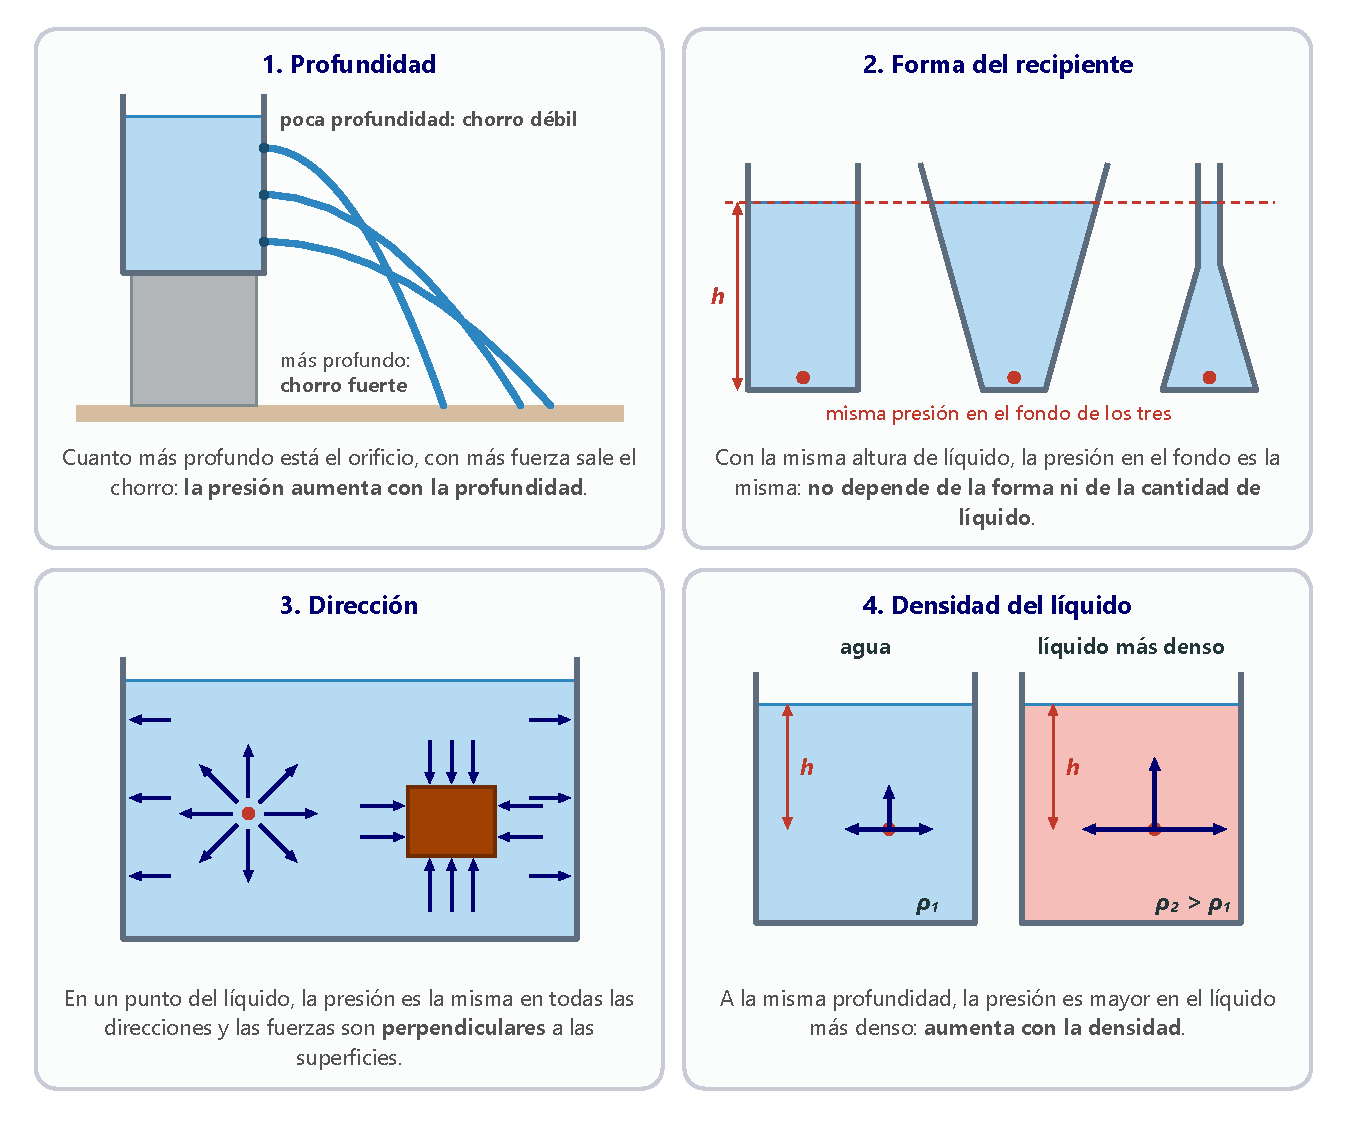
\includegraphics[width=\textwidth]{images/UD10/factores_presion}
    \caption{Factores de los que depende la presión en el interior de un líquido.}
    \label{fig:factores_presion}
\end{figure}

\subsection{¿Cómo se calcula la presión hidrostática?}

Para calcular la presión en un punto A situado a una profundidad \(h\), imaginamos una columna de líquido de base \(S\) que va desde A hasta la superficie libre (figura~\ref{fig:presion_hidrostatica}). La fuerza que actúa sobre la base es el peso de la columna:
\[ F = m \cdot g = \rho \cdot V \cdot g = \rho \cdot S \cdot h \cdot g \]
ya que la masa es \(m = \rho \cdot V\) y el volumen de la columna es \(V = S \cdot h\). Dividiendo entre la superficie:
\[ p = \frac{F}{S} = \frac{\rho \cdot S \cdot h \cdot g}{S} = \rho \cdot g \cdot h \]

\begin{definition}[Presión hidrostática]
    La presión hidrostática a una profundidad \(h\) bajo la superficie libre de un líquido en reposo es igual al producto de la densidad del líquido por la aceleración de la gravedad y por la profundidad:
    \[ p = \rho \cdot g \cdot h \]
\end{definition}

\begin{figure}[H]
    \centering
    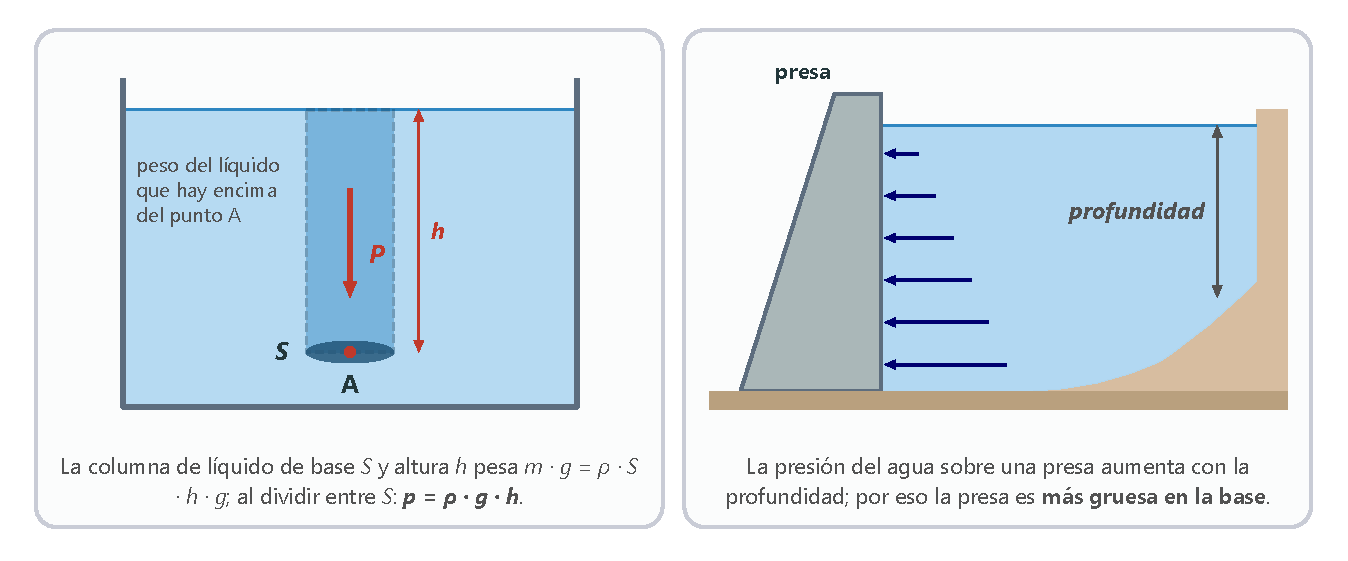
\includegraphics[width=\textwidth]{images/UD10/presion_hidrostatica}
    \caption{Cálculo de la presión hidrostática y presión del agua sobre una presa.}
    \label{fig:presion_hidrostatica}
\end{figure}

La presión hidrostática es \textbf{directamente proporcional} a la profundidad: su gráfica \(p\)--\(h\) es una recta que pasa por el origen, más inclinada cuanto más denso es el líquido.

\begin{center}
    \begin{tikzpicture}
        \begin{axis}[grafica, width=9cm, height=5.6cm, xlabel={profundidad, \(h\) (m)}, ylabel={\(p\) (kPa)}, xmin=0, xmax=10.5, ymin=0, ymax=110, legend pos=north west, legend style={font=\footnotesize}]
            \addplot[mark=none, domain=0:10, line width=1.4pt, color=blue!70!black] {1030*9.8*x/1000};
            \addlegendentry{agua de mar (\qty{1030}{\kg\per\cubic\m})}
            \addplot[mark=none, domain=0:10, line width=1.4pt, color=red!75!black] {800*9.8*x/1000};
            \addlegendentry{aceite (\qty{800}{\kg\per\cubic\m})}
        \end{axis}
    \end{tikzpicture}
\end{center}

\begin{example}
    En una bañera el agua alcanza \qty{35}{\cm} de altura. Calcula la presión hidrostática en el fondo y la fuerza con la que hay que tirar del tapón, circular y de \qty{5}{\cm} de diámetro, para vaciarla.

    \(p = \rho \cdot g \cdot h = 1000 \cdot \num{9.8} \cdot \num{0.35} = \textcolor{red}{\qty{3430}{\pascal}}\).

    La fuerza del agua sobre el tapón es perpendicular a él. Como \(S = \pi \cdot r^2 = \pi \cdot (\num{0.025})^2 = \qty{1.96e-3}{\square\m}\):
    \[ F = p \cdot S = 3430 \cdot \num{1.96e-3} = \textcolor{red}{\qty{6.7}{\newton}} \]
    Para sacar el tapón hay que tirar hacia arriba con una fuerza algo mayor que esta.
\end{example}

\begin{example}
    ¿Por qué el muro de una presa es más grueso en la base que en la parte de arriba?

    Porque la presión del agua \textcolor{red}{aumenta con la profundidad} (figura~\ref{fig:presion_hidrostatica}): la parte baja del muro soporta presiones mucho mayores y necesita más grosor de hormigón para resistirlas.
\end{example}

\begin{exercise}
    Dibuja en tu cuaderno un recipiente con agua y un cuerpo sumergido en ella, y representa las fuerzas que el líquido ejerce sobre las paredes del recipiente y sobre el cuerpo.
    \begin{solu}
        Las fuerzas son \textcolor{red}{perpendiculares} a las paredes y a las caras del cuerpo, dirigidas hacia ellas, y \textcolor{red}{más largas cuanto más profundo} está el punto (como en la figura~\ref{fig:factores_presion}).
    \end{solu}
\end{exercise}

\begin{exercise}
    ¿Qué presión hidrostática soporta un buzo sumergido en el mar a \qty{10}{\m} de profundidad?
    \begin{solu}
        \(p = \rho \cdot g \cdot h = 1030 \cdot \num{9.8} \cdot 10 = \textcolor{red}{\qty{100940}{\pascal}} \approx \qty{1}{\atm}\).
    \end{solu}
\end{exercise}

\begin{exercise}
    El embalse 1 es extenso y poco profundo (\qty{3}{\m}) y contiene más agua que el embalse 2, que es pequeño pero profundo (\qty{6}{\m}). ¿Por qué la presa del embalse 2 tiene que ser más gruesa que la del 1?
    \begin{solu}
        Porque la presión solo depende de la \textcolor{red}{profundidad}, no de la cantidad de agua. En el fondo del embalse 2 la presión es el doble que en el del 1, y su presa necesita \textcolor{red}{más grosor} para soportarla.
    \end{solu}
\end{exercise}

\subsection*{Actividades de consolidación: la presión hidrostática}

\begin{exercise}
    Copia y completa estas frases con las palabras: \emph{perpendicular, direcciones, mayor, mayor, sí depende, no depende}.

    «La presión en el interior de un líquido actúa en todas las \ldots{} y es \ldots{} a las paredes del recipiente. La presión es tanto \ldots{} cuanto \ldots{} es la profundidad; \ldots{} de la densidad del líquido, pero \ldots{} de la forma del recipiente».
    \begin{solu}
        «\ldots{} actúa en todas las \textcolor{red}{direcciones} y es \textcolor{red}{perpendicular} a las paredes del recipiente. La presión es tanto \textcolor{red}{mayor} cuanto \textcolor{red}{mayor} es la profundidad; \textcolor{red}{sí depende} de la densidad del líquido, pero \textcolor{red}{no depende} de la forma del recipiente».
    \end{solu}
\end{exercise}

\begin{exercise}
    ¿Qué presión ejerce sobre su base un prisma de hierro de \qty{20}{\cm} de altura y \qty{10}{\square\cm} de base? Dato: \(\rho_{\text{hierro}} = \qty{7800}{\kg\per\cubic\m}\). ¿Depende el resultado del área de la base?
    \begin{solu}
        \(p = \dfrac{P}{S} = \dfrac{\rho \cdot S \cdot h \cdot g}{S} = \rho \cdot g \cdot h = 7800 \cdot \num{9.8} \cdot \num{0.20} = \textcolor{red}{\qty{1.53e4}{\pascal}}\).
        \textcolor{red}{No depende del área} de la base, igual que la presión hidrostática no depende de la forma del recipiente.
    \end{solu}
\end{exercise}

\begin{exercise}
    Responde verdadero o falso y justifica tu respuesta:
    \begin{enumerate}[label=\alph*)]
        \item La presión en el interior de un líquido es mayor cuanto menor es su densidad.
        \item La presión es directamente proporcional a la anchura del recipiente.
        \item La presión es directamente proporcional a la profundidad.
        \item La presión en el interior de un líquido actúa en todas las direcciones.
    \end{enumerate}
    \begin{solu}
        a) \textcolor{red}{Falso}: es mayor cuanto mayor es la densidad. b) \textcolor{red}{Falso}: no depende de la anchura. c) \textcolor{red}{Verdadero}. d) \textcolor{red}{Verdadero}.
    \end{solu}
\end{exercise}

\begin{exercise}
    Tenemos cuatro recipientes de la misma altura llenos hasta arriba: A y B tienen la misma forma, pero A contiene agua y B mercurio; C y D contienen agua, pero D es mucho más estrecho que C. ¿Por qué la presión del mercurio sobre las paredes de B es mayor que la del agua sobre las paredes de A? ¿Por qué es la misma en C y en D?
    \begin{solu}
        En B la presión es mayor porque la \textcolor{red}{densidad del mercurio es mayor} que la del agua. En C y D es la misma porque contienen el mismo líquido y tienen la \textcolor{red}{misma profundidad}; la anchura no influye.
    \end{solu}
\end{exercise}

\begin{exercise}
    Toma un tubo de vidrio abierto por los dos extremos y tapa uno de ellos con una placa de plástico sujeta con un hilo tenso.
    \begin{enumerate}[label=\alph*)]
        \item Introduce el tubo en una cubeta con agua, con la placa hacia abajo. ¿Qué ocurre al soltar el hilo?
        \item Ahora echa agua dentro del tubo poco a poco. ¿Qué sucede cuando el nivel del agua del tubo alcanza el de la cubeta?
    \end{enumerate}
    \begin{solu}
        a) La placa \textcolor{red}{no se cae}: el agua de la cubeta la empuja hacia arriba (y lo hace en cualquier orientación del tubo).
        b) La placa \textcolor{red}{se desprende}, porque la presión del agua por dentro y por fuera es la misma y su propio peso la hace caer.
    \end{solu}
\end{exercise}

\begin{exercise}
    Calcula la presión en el fondo de un recipiente de \qty{76}{\cm} de profundidad cuando se llena de agua y cuando se llena de mercurio (\(\rho = \qty{13600}{\kg\per\cubic\m}\)).
    \begin{solu}
        Agua: \(p = 1000 \cdot \num{9.8} \cdot \num{0.76} = \textcolor{red}{\qty{7448}{\pascal}}\).
        Mercurio: \(p = 13600 \cdot \num{9.8} \cdot \num{0.76} = \textcolor{red}{\qty{1.013e5}{\pascal}}\), que es justo la presión atmosférica normal.
    \end{solu}
\end{exercise}

\begin{exercise}
    Una piscina tiene \qty{1}{\m} de profundidad en la zona menos profunda y \qty{2}{\m} en la más profunda. Calcula la presión del agua en el fondo de cada zona.
    \begin{solu}
        Zona profunda: \(p = 1000 \cdot \num{9.8} \cdot 2 = \textcolor{red}{\qty{19600}{\pascal}}\). Zona menos profunda: \(p = 1000 \cdot \num{9.8} \cdot 1 = \textcolor{red}{\qty{9800}{\pascal}}\).
    \end{solu}
\end{exercise}

\begin{exercise}
    Un batiscafo desciende en el océano hasta \qty{150}{\m} de profundidad. Si la densidad del agua es \qty{1040}{\kg\per\cubic\m}, calcula la presión hidrostática a esa profundidad y la fuerza que soporta una ventanilla circular de \qty{40}{\cm} de diámetro.
    \begin{solu}
        \(p = 1040 \cdot \num{9.8} \cdot 150 = \textcolor{red}{\qty{1.53e6}{\pascal}}\).
        \(S = \pi \cdot \num{0.20}^2 = \qty{0.126}{\square\m}\); \(F = p \cdot S = \num{1.53e6} \cdot \num{0.126} = \textcolor{red}{\qty{1.92e5}{\newton}}\) (como el peso de unas 20 toneladas).
    \end{solu}
\end{exercise}

\begin{exercise}
    Un submarino está sumergido a \qty{300}{\m} de profundidad en agua de mar. Calcula:
    \begin{enumerate}[label=\alph*)]
        \item La presión hidrostática sobre él, en pascales y en atmósferas.
        \item La fuerza que actúa sobre una de sus compuertas, de \qty{4.2}{\square\m}.
    \end{enumerate}
    \begin{solu}
        a) \(p = 1030 \cdot \num{9.8} \cdot 300 = \textcolor{red}{\qty{3.03e6}{\pascal}}\); \(\dfrac{\num{3.03e6}}{\num{1.013e5}} = \textcolor{red}{\qty{29.9}{\atm}}\).
        b) \(F = p \cdot S = \num{3.03e6} \cdot \num{4.2} = \textcolor{red}{\qty{1.27e7}{\newton}}\).
    \end{solu}
\end{exercise}

\begin{exercise}
    ¿Qué fuerza total soporta un buzo sumergido en el mar a \qty{8}{\m} de profundidad, si la superficie de su cuerpo es de \qty{150}{\square\dm}?
    \begin{solu}
        \(p = 1030 \cdot \num{9.8} \cdot 8 = \qty{80752}{\pascal}\). La superficie es \(\qty{150}{\square\dm} = \qty{1.5}{\square\m}\), así que
        \(F = p \cdot S = 80752 \cdot \num{1.5} = \textcolor{red}{\qty{1.21e5}{\newton}}\).
    \end{solu}
\end{exercise}

%========================================================================================
\section{Principio fundamental de la hidrostática}
%========================================================================================

Consideremos dos puntos A y B en el interior de un líquido en reposo, a las profundidades \(h_A\) y \(h_B\) (figura~\ref{fig:principio_fundamental}). Las presiones en ellos son \(p_A = \rho \cdot g \cdot h_A\) y \(p_B = \rho \cdot g \cdot h_B\), así que su diferencia es:
\[ p_A - p_B = \rho \cdot g \cdot (h_A - h_B) \]

\begin{definition}[Principio fundamental de la hidrostática]
    La \textbf{diferencia de presión entre dos puntos} de un fluido homogéneo en equilibrio es igual al producto de la densidad por la aceleración de la gravedad y por la diferencia de profundidad entre ellos:
    \[ \Delta p = \rho \cdot g \cdot \Delta h \]
\end{definition}

Una consecuencia importante: \textbf{todos los puntos de un líquido que están a la misma profundidad soportan la misma presión}, sea cual sea la forma del recipiente.

\begin{figure}[H]
    \centering
    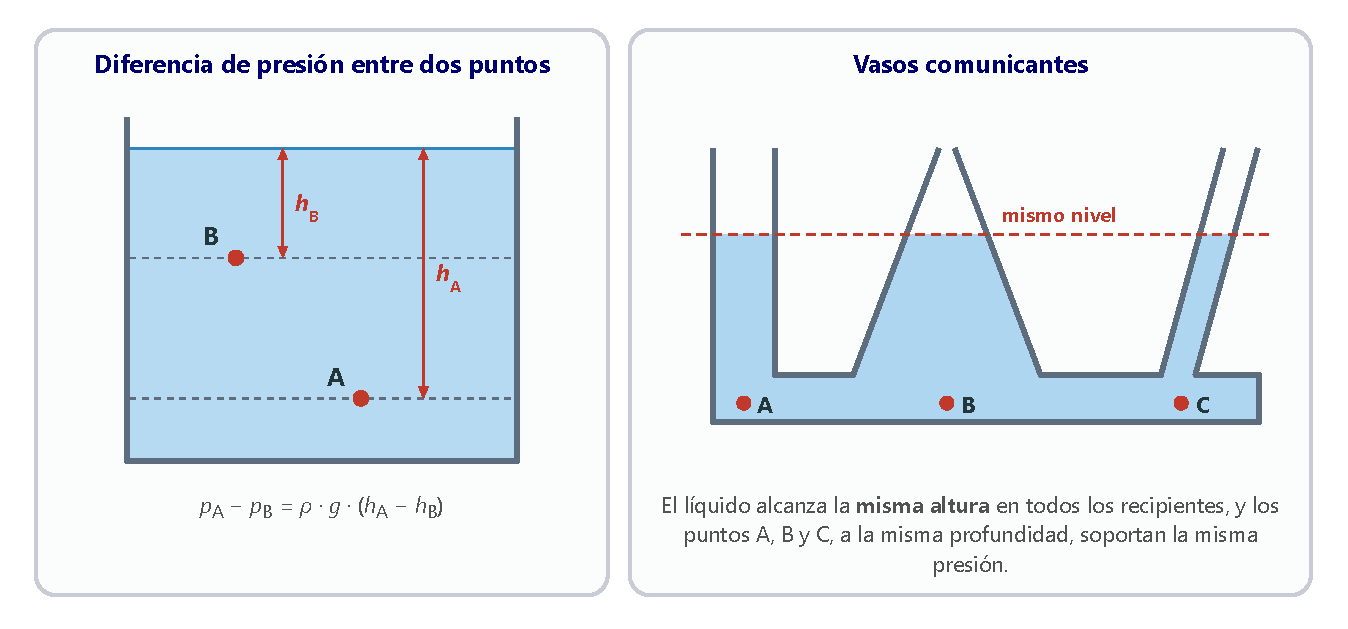
\includegraphics[width=\textwidth]{images/UD10/principio_fundamental}
    \caption{Principio fundamental de la hidrostática y vasos comunicantes.}
    \label{fig:principio_fundamental}
\end{figure}

\begin{example}
    Calcula la diferencia de presión entre dos puntos de un líquido de densidad \qty{1500}{\kg\per\cubic\m} situados a \qty{10}{\cm} y a \qty{30}{\cm} por debajo de la superficie libre.
    \[ p_A - p_B = \rho \cdot g \cdot (h_A - h_B) = 1500 \cdot \num{9.8} \cdot (\num{0.30} - \num{0.10}) = \textcolor{red}{\qty{2940}{\pascal}} \]
\end{example}

\subsection{¿Qué son los vasos comunicantes?}

Los \textbf{vasos comunicantes} son varios recipientes, de igual o distinta forma, abiertos por arriba y comunicados entre sí por la base. Si se vierte un líquido en uno de ellos, \textbf{alcanza la misma altura en todos} (figura~\ref{fig:principio_fundamental}).

Según el principio fundamental, la forma no influye: si el líquido estuviera más alto en un recipiente, la presión en su base sería mayor que en la de los demás y el líquido fluiría hasta igualar las alturas. Así funcionan el abastecimiento de agua de las ciudades desde depósitos elevados, los niveles de agua que usan los albañiles o las esclusas de los canales.

\begin{exercise}
    Una aplicación de los vasos comunicantes es el abastecimiento de agua a las ciudades.
    \begin{enumerate}[label=\alph*)]
        \item Busca información sobre cómo se abastece de agua una ciudad mediante depósitos.
        \item Justifica por qué el depósito debe estar a mayor altura que los edificios.
    \end{enumerate}
    \begin{solu}
        a) Respuesta libre. El agua se almacena en depósitos situados en lugares altos y llega a las casas por tuberías conectadas con ellos.
        b) La red de tuberías y el depósito forman unos \textcolor{red}{vasos comunicantes}: el agua tiende a alcanzar en las tuberías la misma altura que en el depósito. Para que llegue con presión suficiente a los pisos más altos, el depósito tiene que estar \textcolor{red}{por encima del edificio más alto}.
    \end{solu}
\end{exercise}

\begin{exercise}
    ¿Qué diferencia de presión hay entre dos puntos situados a \qty{1}{\m} y a \qty{10}{\m} por debajo de la superficie del agua?
    \begin{solu}
        \(\Delta p = \rho \cdot g \cdot \Delta h = 1000 \cdot \num{9.8} \cdot 9 = \textcolor{red}{\qty{88200}{\pascal}}\).
    \end{solu}
\end{exercise}

\subsection*{Actividades de consolidación: principio fundamental de la hidrostática}

\begin{exercise}
    ¿Qué diferencia de presión hay entre dos puntos situados a \qty{10}{\cm} y a \qty{35}{\cm} por debajo del nivel del agua?
    \begin{solu}
        \(\Delta p = 1000 \cdot \num{9.8} \cdot \num{0.25} = \textcolor{red}{\qty{2450}{\pascal}}\).
    \end{solu}
\end{exercise}

\begin{exercise}
    ¿A qué profundidad hay que sumergirse en un embalse para que la presión total que se soporta sea el doble que en la superficie? (En la superficie la presión es la atmosférica, \qty{1.013e5}{\pascal}).
    \begin{solu}
        La presión total será el doble cuando la presión hidrostática del agua sea igual a la atmosférica:
        \[ \num{1.013e5} = 1000 \cdot \num{9.8} \cdot h \quad\Rightarrow\quad h = \textcolor{red}{\qty{10.3}{\m}} \]
    \end{solu}
\end{exercise}

\begin{exercise}
    ¿Qué diferencia de presión hay entre dos puntos de un líquido de densidad \qty{1800}{\kg\per\cubic\m} separados por una distancia vertical de \qty{20}{\cm}?
    \begin{solu}
        \(\Delta p = 1800 \cdot \num{9.8} \cdot \num{0.20} = \textcolor{red}{\qty{3528}{\pascal}}\).
    \end{solu}
\end{exercise}

\begin{exercise}
    Si se ponen en comunicación vasijas de distintos tamaños y formas y se vierte un líquido en ellas, ¿cómo serán los niveles que alcanza el líquido?
    \begin{solu}
        El líquido alcanza el \textcolor{red}{mismo nivel en todas} las vasijas.
    \end{solu}
\end{exercise}

\begin{exercise}
    Un depósito cúbico de \qty{150}{\cm} de arista está lleno de agua. Calcula:
    \begin{enumerate}[label=\alph*)]
        \item La presión hidrostática en el fondo.
        \item La fuerza que ejerce el agua sobre el fondo.
        \item La presión en un punto situado a \qty{75}{\cm} de profundidad.
    \end{enumerate}
    \begin{solu}
        a) \(p = 1000 \cdot \num{9.8} \cdot \num{1.5} = \textcolor{red}{\qty{14700}{\pascal}}\).
        b) \(F = p \cdot S = 14700 \cdot \num{1.5}^2 = \textcolor{red}{\qty{33075}{\newton}}\) (coincide con el peso del agua del depósito).
        c) \(p = 1000 \cdot \num{9.8} \cdot \num{0.75} = \textcolor{red}{\qty{7350}{\pascal}}\).
    \end{solu}
\end{exercise}

%========================================================================================
\section{Principio de Pascal}
%========================================================================================

Si llenamos de agua una jeringa con un globo agujereado en la punta y empujamos el émbolo, el agua sale con la misma fuerza por todos los agujeros (figura~\ref{fig:pascal_prensa}). La presión que ejercemos con el émbolo se transmite a todo el líquido. En el siglo \textsc{xvii}, el científico francés \textbf{Blaise Pascal} lo enunció así:

\begin{definition}[Principio de Pascal]
    La presión ejercida en un punto de un \textbf{líquido incompresible} encerrado en un recipiente se transmite \textbf{por igual} a todos los puntos del líquido y a las paredes del recipiente, en todas las direcciones.
\end{definition}

\subsection{¿Qué aplicaciones tiene el principio de Pascal? La prensa hidráulica}

En el principio de Pascal se basan la prensa hidráulica, el gato y el elevador hidráulicos de los talleres, los frenos hidráulicos de los coches o las excavadoras.

La \textbf{prensa hidráulica} está formada por dos cilindros de secciones distintas, \(S_1\) (pequeña) y \(S_2\) (grande), unidos por un tubo y llenos de un líquido. Cada cilindro está cerrado por un émbolo. La presión que ejerce el émbolo pequeño se transmite sin variación al grande:
\[ p_1 = p_2 \quad\Rightarrow\quad \frac{F_1}{S_1} = \frac{F_2}{S_2} \quad\Rightarrow\quad F_2 = F_1 \cdot \frac{S_2}{S_1} \]
La fuerza que aparece en el émbolo grande es la aplicada en el pequeño \textbf{multiplicada por el cociente de las secciones}, \(S_2/S_1\). Cuanto mayor es la diferencia de tamaño de los émbolos, más eficaz es la prensa.

\begin{figure}[H]
    \centering
    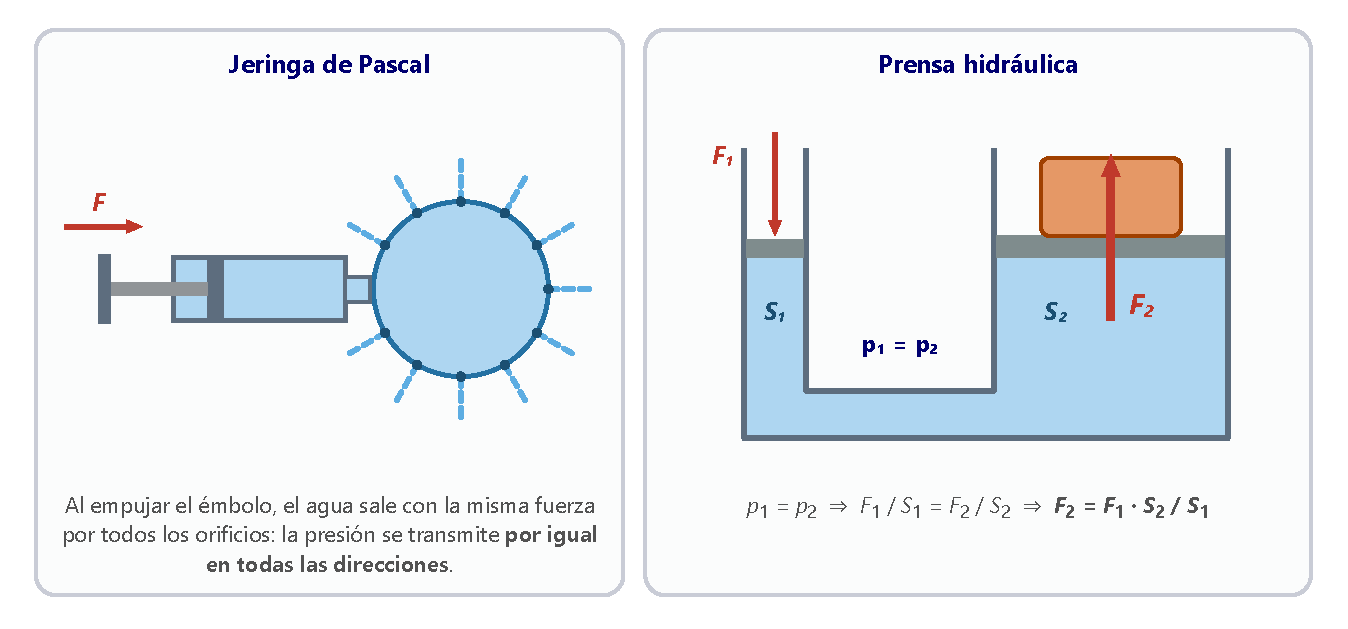
\includegraphics[width=\textwidth]{images/UD10/pascal_prensa}
    \caption{El principio de Pascal y la prensa hidráulica.}
    \label{fig:pascal_prensa}
\end{figure}

\begin{example}
    Los émbolos de una prensa hidráulica tienen \qty{1}{\cm} y \qty{10}{\cm} de radio. Sobre el pequeño se ejerce una fuerza de \qty{500}{\newton}. ¿Qué fuerza aparece en el grande?

    \(S_1 = \pi \cdot (\num{0.01})^2 = \qty{3.14e-4}{\square\m}\); \quad \(S_2 = \pi \cdot (\num{0.10})^2 = \qty{3.14e-2}{\square\m}\).
    \[ F_2 = F_1 \cdot \frac{S_2}{S_1} = 500 \cdot \frac{\num{3.14e-2}}{\num{3.14e-4}} = \textcolor{red}{\qty{5e4}{\newton}} \]
    Con \qty{500}{\newton} se pueden levantar unos \qty{5000}{\kg}: al multiplicar el radio por 10, la superficie (y la fuerza) se multiplica por 100.
\end{example}

\begin{exercise}
    ¿Qué superficie debe tener el émbolo grande de una prensa hidráulica para que, al ejercer \qty{20}{\newton} sobre el pequeño (de \qty{10}{\square\cm}), aparezca en el grande una fuerza de \qty{2000}{\newton}?
    \begin{solu}
        \(S_2 = S_1 \cdot \dfrac{F_2}{F_1} = 10 \cdot \dfrac{2000}{20} = \textcolor{red}{\qty{1000}{\square\cm}}\).
    \end{solu}
\end{exercise}

\subsection*{Actividades de consolidación: principio de Pascal}

\begin{exercise}
    Con una prensa hidráulica obtenemos una fuerza diez veces mayor que la que aplicamos. ¿Qué relación hay entre las secciones de los émbolos?
    \begin{solu}
        La sección del émbolo grande es \textcolor{red}{diez veces mayor} que la del pequeño.
    \end{solu}
\end{exercise}

\begin{exercise}
    La sección del émbolo grande de una prensa hidráulica es cien veces mayor que la del pequeño. ¿Qué fuerza actúa sobre el grande si sobre el pequeño se ejercen \qty{50}{\newton}?
    \begin{solu}
        \(F_2 = 50 \cdot 100 = \textcolor{red}{\qty{5000}{\newton}}\).
    \end{solu}
\end{exercise}

\begin{exercise}
    Un mecánico dice que su prensa hidráulica levanta camiones de hasta \qty{8000}{\kg}. La fuerza máxima que se puede aplicar sobre el émbolo pequeño es de \qty{2500}{\newton} y los diámetros de los émbolos son \qty{10}{\cm} y \qty{50}{\cm}. ¿Es cierto lo que dice?
    \begin{solu}
        Como \(S = \pi \cdot d^2/4\), el cociente de secciones es el cuadrado del cociente de diámetros: \(\dfrac{S_2}{S_1} = \left(\dfrac{50}{10}\right)^2 = 25\).
        \(F_2 = 2500 \cdot 25 = \qty{62500}{\newton}\), y el peso del camión es \(8000 \cdot \num{9.8} = \qty{78400}{\newton}\). \textcolor{red}{No es cierto}: como máximo levanta unos \qty{6400}{\kg}.
    \end{solu}
\end{exercise}

\begin{exercise}
    Queremos levantar con un elevador hidráulico una furgoneta que pesa \qty{20000}{\newton}. La sección del émbolo menor es de \qty{10}{\square\cm} y la del mayor, de \qty{140}{\square\cm}. ¿Qué fuerza hay que aplicar sobre el émbolo pequeño?
    \begin{solu}
        \(F_1 = F_2 \cdot \dfrac{S_1}{S_2} = 20000 \cdot \dfrac{10}{140} = \textcolor{red}{\qty{1429}{\newton}}\).
    \end{solu}
\end{exercise}

\begin{exercise}
    Busca información sobre cómo funcionan los frenos ABS de los coches y cómo deben usarlos los conductores. ¿El ABS aumenta o disminuye la distancia de frenado?
    \begin{solu}
        Respuesta libre. El ABS (\emph{sistema antibloqueo de frenos}) controla la presión del líquido de frenos para que las ruedas \textcolor{red}{no se bloqueen} al frenar: los neumáticos no pierden adherencia y el conductor puede frenar y girar a la vez. Hay que pisar el freno a fondo y mantenerlo pisado. En general, sobre todo en suelo mojado, \textcolor{red}{reduce la distancia de frenado} y evita derrapes.
    \end{solu}
\end{exercise}

%========================================================================================
\section[La presión atmosférica]{¿Ejerce la atmósfera presión sobre los cuerpos que están en su interior? La presión atmosférica}
%========================================================================================

Vivimos en el fondo de un «océano» de aire, la atmósfera, que tiene más de \qty{100}{\km} de espesor. Como cualquier fluido, el aire ejerce una presión sobre los cuerpos que hay en él, debida a su peso: es la \textbf{presión atmosférica}. Algunas experiencias cotidianas la ponen de manifiesto (figura~\ref{fig:presion_atmosferica}):
\begin{itemize}
    \item Al sorber con una pajita, sacamos el aire de su interior; la presión atmosférica, que actúa sobre la superficie del líquido del vaso, lo empuja hacia arriba por la pajita.
    \item Si llenamos un vaso de agua, lo tapamos con una cartulina y le damos la vuelta, el agua no cae: la presión atmosférica empuja la cartulina desde abajo.
    \item Las ventosas se quedan pegadas a una superficie lisa porque, al apretarlas, sale el aire de su interior y la presión atmosférica las aprieta desde fuera.
\end{itemize}

\begin{figure}[H]
    \centering
    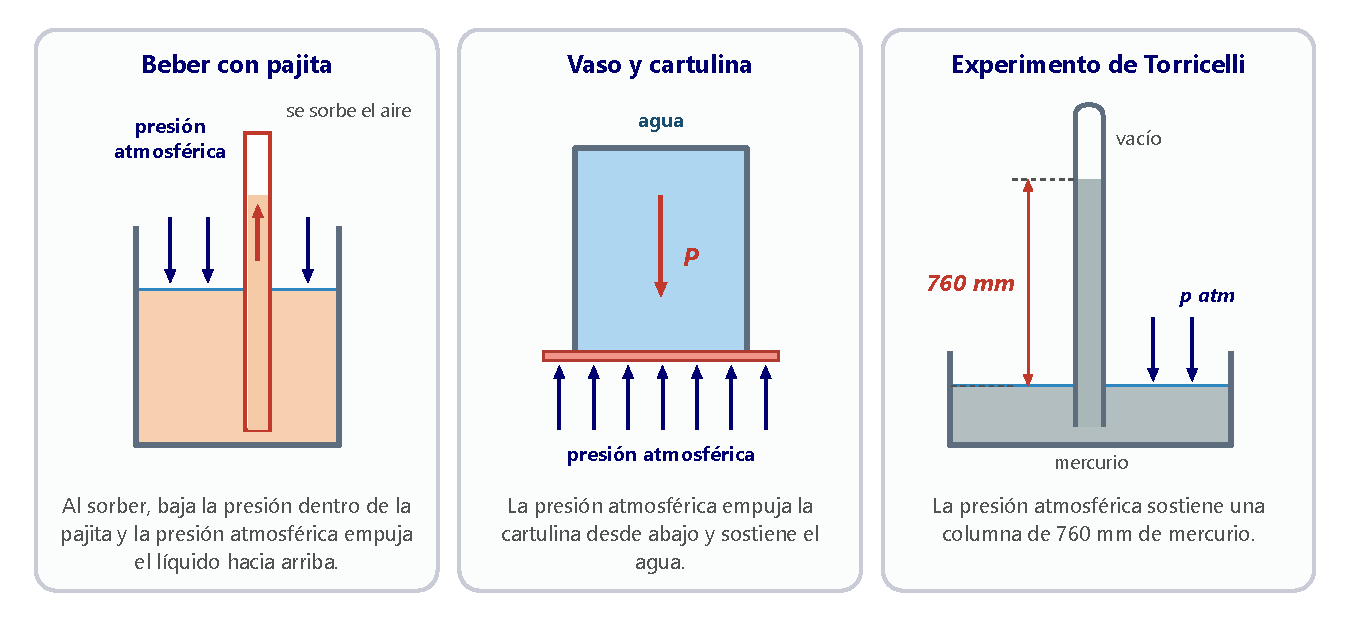
\includegraphics[width=\textwidth]{images/UD10/presion_atmosferica}
    \caption{Tres experiencias que muestran la presión atmosférica.}
    \label{fig:presion_atmosferica}
\end{figure}

\subsection{¿Cómo se mide la presión atmosférica?}

En 1643, el italiano \textbf{Evangelista Torricelli} llenó de mercurio un tubo de vidrio de \qty{1}{\m} de longitud, cerrado por un extremo. Tapó con el dedo el extremo abierto, le dio la vuelta y lo introdujo en una cubeta con mercurio. Al quitar el dedo, el mercurio del tubo bajó hasta quedar a \qty{760}{\mm} por encima del nivel de la cubeta, dejando vacío en la parte de arriba (figura~\ref{fig:presion_atmosferica}).

La columna no baja más porque la presión atmosférica, que actúa sobre el mercurio de la cubeta, la sostiene: la presión que ejerce la columna de mercurio es igual a la presión atmosférica.

\begin{definition}[Presión atmosférica normal]
    La presión que ejerce una columna de mercurio de \qty{760}{\mm} de altura se llama \textbf{presión atmosférica normal}, y para medirla se usa una unidad llamada \textbf{atmósfera} (\unit{\atm}):
    \[ \qty{1}{\atm} = \qty{760}{\mmHg} = \qty{1.013e5}{\pascal} \]
    La presión atmosférica se mide con un \textbf{barómetro}.
\end{definition}

Podemos comprobar la equivalencia con la presión hidrostática de la columna: \(p = \rho \cdot g \cdot h = 13600 \cdot \num{9.8} \cdot \num{0.760} = \qty{1.013e5}{\pascal}\).

La altura de la columna no depende de la longitud ni de la sección del tubo, ni de su inclinación: solo de la presión atmosférica del lugar.

\subsection{¿Qué relación hay entre la presión atmosférica y la altitud?}

Cuanto más subimos, menos aire tenemos encima y \textbf{menor es la presión atmosférica}. Además, el aire de las capas altas está menos comprimido y es menos denso, por lo que la presión no disminuye de forma proporcional a la altitud: cerca del nivel del mar hay que subir unos \qty{10}{\m} para que la presión baje \qty{1}{\mmHg}, pero a \qty{5000}{\m} de altitud hay que subir unos \qty{20}{\m}.

\begin{center}
    \begin{tikzpicture}
        \begin{axis}[grafica, width=10cm, height=6cm, xlabel={altitud (km)}, ylabel={presión (mmHg)}, xmin=0, xmax=12.5, ymin=0, ymax=800, xtick={0,2,...,12}]
            \addplot[mark=none, domain=0:12, samples=60, line width=1.4pt, color=red!75!black] {760*(1-0.022558*x)^5.256};
            \addplot[only marks, mark=*, mark size=2pt, color=blue!70!black] coordinates {(0,760) (5.5,380) (8.849,236)};
            \node[font=\scriptsize, anchor=west] at (axis cs:0.4,740) {nivel del mar: 760};
            \node[font=\scriptsize, anchor=south west] at (axis cs:5.6,382) {\qty{5500}{\m}: la mitad};
            \node[font=\scriptsize, anchor=south west] at (axis cs:8.9,238) {cima del Everest};
        \end{axis}
    \end{tikzpicture}
\end{center}

Por eso, a gran altura cuesta respirar (hay menos oxígeno en cada inspiración), el agua hierve a menos de \qty{100}{\degreeCelsius} y las cabinas de los aviones tienen que estar presurizadas. Los \textbf{altímetros} de los aviones son barómetros graduados en metros.

\subsection{Previsión del tiempo: borrascas y anticiclones}

En meteorología se usan como unidades de presión el \textbf{milibar} (mb) y el \textbf{hectopascal} (\unit{\hecto\pascal}), que son equivalentes: \(\qty{1}{\hecto\pascal} = \qty{100}{\pascal} = 1~\text{mb}\). El valor medio de la presión atmosférica a nivel del mar es de unos \qty{1013}{\hecto\pascal}; las presiones superiores se llaman \emph{altas} y las inferiores, \emph{bajas}.

\paragraph{¿Qué es un mapa meteorológico?} Es un mapa en el que se representan los valores de la presión atmosférica medidos a la vez en muchas estaciones meteorológicas; se usa para predecir el tiempo. Las \textbf{isobaras} son líneas que unen los puntos de igual presión, y suelen trazarse cada \qty{4}{\hecto\pascal}. Si están muy juntas, hay vientos fuertes; si están separadas, los vientos son suaves. Con una \textbf{A} se marcan los \textbf{anticiclones}, zonas de altas presiones, y con una \textbf{B}, las \textbf{borrascas}, zonas de bajas presiones (figura~\ref{fig:borrascas_anticiclones}).

\paragraph{¿Cómo se forman las borrascas y los anticiclones?} Se deben a las diferencias de temperatura en la atmósfera:
\begin{itemize}
    \item Si el aire está \textbf{frío}, es más denso y \textbf{desciende}, creando una zona de altas presiones: un \textbf{anticiclón}. Al llegar al suelo, el aire se separa (corrientes divergentes) y no se mezclan masas de aire distintas: el tiempo suele ser \textbf{bueno y estable}. En el hemisferio norte, el aire de un anticiclón gira en el sentido de las agujas del reloj.
    \item Si el aire está \textbf{caliente}, es menos denso y \textbf{asciende}, dejando debajo una zona de bajas presiones: una \textbf{borrasca}. El aire de los alrededores converge hacia ella, se mezclan masas de aire de distinto origen y, al subir, el vapor de agua se condensa: el tiempo suele ser \textbf{inestable}, con nubes y lluvias. En el hemisferio norte, el aire de una borrasca gira en sentido contrario al de las agujas del reloj.
\end{itemize}
En todos los casos el aire se desplaza desde las zonas de alta presión hasta las de baja presión: son las \textbf{corrientes de viento}. Las borrascas y los anticiclones no están quietos, sino que se desplazan y cambian de forma.

\begin{figure}[H]
    \centering
    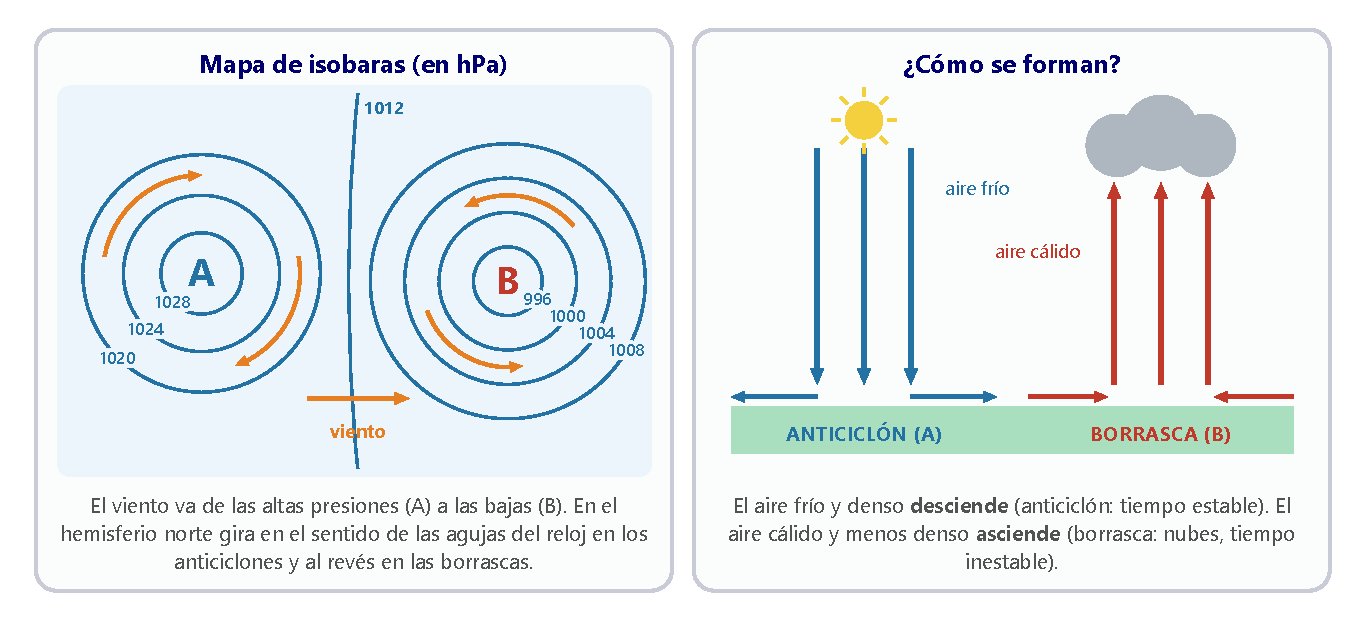
\includegraphics[width=\textwidth]{images/UD10/borrascas_anticiclones}
    \caption{Isobaras, anticiclones y borrascas.}
    \label{fig:borrascas_anticiclones}
\end{figure}

\paragraph{¿Qué diferencia hay entre un frente frío y uno cálido?} En la atmósfera hay \textbf{masas de aire frío}, más frías que la superficie sobre la que avanzan, y \textbf{masas de aire cálido}, más calientes. La zona de separación entre dos masas de aire distintas es una \textbf{superficie frontal}, y su intersección con el suelo es un \textbf{frente} (figura~\ref{fig:frentes}):
\begin{itemize}
    \item En un \textbf{frente frío}, el aire frío empuja al cálido y lo obliga a subir rápidamente; se forman nubes de gran desarrollo vertical y chubascos. En los mapas se dibuja con una línea de \textbf{triángulos} que apuntan en el sentido de avance.
    \item En un \textbf{frente cálido}, una masa de aire templado avanza y sube lentamente sobre el aire frío, que retrocede; se forman nubes extensas y lluvias débiles. Se dibuja con una línea de \textbf{semicírculos}.
\end{itemize}

\begin{figure}[H]
    \centering
    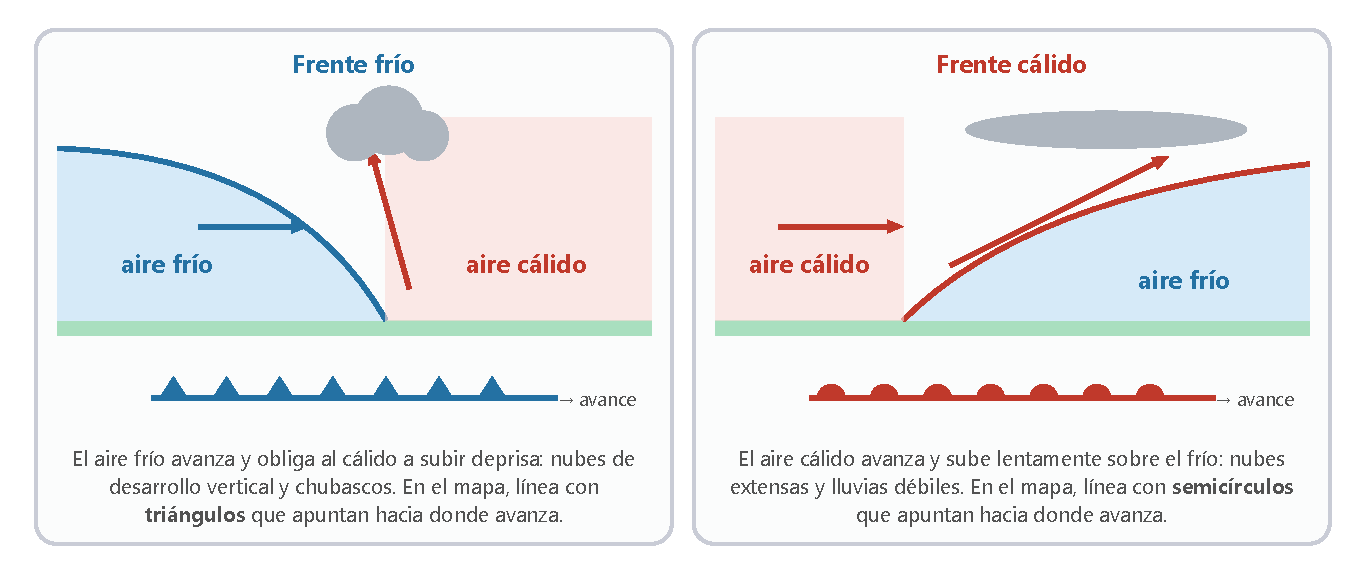
\includegraphics[width=\textwidth]{images/UD10/frentes}
    \caption{Frente frío y frente cálido, y sus símbolos en los mapas del tiempo.}
    \label{fig:frentes}
\end{figure}

\begin{exercise}
    La presión del aire dentro de un neumático es de \qty{1.25}{\atm}. Exprésala en milímetros de mercurio y en pascales.
    \begin{solu}
        \(\num{1.25}~\unit{\atm} \cdot \dfrac{\qty{760}{\mmHg}}{\qty{1}{\atm}} = \textcolor{red}{\qty{950}{\mmHg}}\); \quad \(\num{1.25}~\unit{\atm} \cdot \dfrac{\qty{1.013e5}{\pascal}}{\qty{1}{\atm}} = \textcolor{red}{\qty{1.27e5}{\pascal}}\).
    \end{solu}
\end{exercise}

\begin{exercise}
    ¿Por qué las cabinas de los aviones están selladas y presurizadas?
    \begin{solu}
        Porque a la altura a la que vuelan los aviones (unos \qty{10}{\km}) la \textcolor{red}{presión atmosférica es muy baja}, alrededor de una cuarta parte de la del nivel del mar, y no podríamos respirar bien. La cabina mantiene dentro una \textcolor{red}{presión mucho mayor} que la exterior, parecida a la que hay a unos \qty{2000}{\m} de altitud.
    \end{solu}
\end{exercise}

\begin{exercise}
    Un barómetro marca \qty{745}{\mmHg} en una localidad costera. ¿Hay una borrasca o un anticiclón sobre ella? ¿Qué tiempo cabe esperar?
    \begin{solu}
        Marca menos de \qty{760}{\mmHg} (\(745 \cdot \num{1.333} \approx \qty{993}{\hecto\pascal}\), por debajo de \qty{1013}{\hecto\pascal}): hay una \textcolor{red}{borrasca}, y cabe esperar \textcolor{red}{tiempo inestable}, con nubes y probablemente lluvia.
    \end{solu}
\end{exercise}

\begin{exercise}
    En un mapa del tiempo, la isobara más exterior que rodea un anticiclón es de \qty{1016}{\hecto\pascal}, y la más exterior que rodea una borrasca es de \qty{1004}{\hecto\pascal}. Si en el interior de cada uno hay dos isobaras más, trazadas cada \qty{4}{\hecto\pascal}, ¿qué valores tienen?
    \begin{solu}
        En el anticiclón la presión aumenta hacia el centro: \textcolor{red}{\qty{1020}{\hecto\pascal} y \qty{1024}{\hecto\pascal}}. En la borrasca disminuye hacia el centro: \textcolor{red}{\qty{1000}{\hecto\pascal} y \qty{996}{\hecto\pascal}}.
    \end{solu}
\end{exercise}

\subsection*{Actividades de consolidación: la presión atmosférica}

\begin{exercise}
    Asocia cada concepto con sus características (un concepto puede tener varias):

    \textbf{Conceptos:} a) presión atmosférica; b) isobaras; c) anticiclones; d) borrascas; e) corrientes de viento; f) frente frío; g) frente cálido.

    \textbf{Características:} 1. Línea con semicírculos. 2. Se mide con un barómetro. 3. Línea con triángulos. 4. Se expresa en atm, mmHg y Pa. 5. Líneas que unen puntos de igual presión. 6. Disminuye con la altitud. 7. Zonas de baja presión. 8. Zonas de alta presión. 9. Tiempo estable. 10. Tiempo inestable. 11. El aire va de las altas a las bajas presiones.
    \begin{solu}
        a) \textcolor{red}{2, 4 y 6}; b) \textcolor{red}{5}; c) \textcolor{red}{8 y 9}; d) \textcolor{red}{7 y 10}; e) \textcolor{red}{11}; f) \textcolor{red}{3}; g) \textcolor{red}{1}.
    \end{solu}
\end{exercise}

\begin{exercise}
    ¿Se puede usar un barómetro para calcular la altura de una montaña? Busca información sobre cómo funciona un altímetro.
    \begin{solu}
        \textcolor{red}{Sí}, porque la presión atmosférica disminuye con la altitud de forma conocida. Un \textcolor{red}{altímetro} es un barómetro graduado en metros: mide la presión y la convierte en la diferencia de altitud respecto a un lugar de referencia, normalmente el nivel del mar.
    \end{solu}
\end{exercise}

\begin{exercise}
    Si en el experimento de Torricelli se usara agua en lugar de mercurio, ¿qué altura alcanzaría el agua en el tubo?
    \begin{solu}
        \(\num{1.013e5} = 1000 \cdot \num{9.8} \cdot h \Rightarrow h = \textcolor{red}{\qty{10.3}{\m}}\). Haría falta un tubo de más de diez metros: por eso se usa mercurio, que es 13,6 veces más denso.
    \end{solu}
\end{exercise}

\begin{exercise}
    Si la densidad del aire fuera constante e igual a \qty{1.2}{\kg\per\cubic\m}, ¿qué altura tendría que tener la atmósfera para ejercer una presión de \qty{1.013e5}{\pascal}?
    \begin{solu}
        \(\num{1.013e5} = \num{1.2} \cdot \num{9.8} \cdot h \Rightarrow h = \textcolor{red}{\qty{8614}{\m}}\). La atmósfera real es mucho más alta porque su densidad disminuye con la altitud.
    \end{solu}
\end{exercise}

\begin{exercise}
    En una cubeta con mercurio se colocan tres tubos de un metro, cerrados por arriba y llenos de mercurio: uno vertical, otro inclinado y otro más ancho. ¿A qué altura vertical sobre el nivel de la cubeta quedará el mercurio en cada uno? ¿Por qué?
    \begin{solu}
        En los tres, a \textcolor{red}{\qty{760}{\mm}} de altura vertical (a nivel del mar). La presión atmosférica sobre la cubeta sostiene una columna cuya altura vertical \textcolor{red}{no depende de la forma, la sección ni la inclinación} del tubo (en el inclinado, el mercurio recorre más longitud de tubo, pero llega a la misma altura).
    \end{solu}
\end{exercise}

\begin{exercise}
    Una persona con una superficie corporal de \qty{1.5}{\square\m} soporta, por la presión atmosférica, una fuerza equivalente al peso de unas 15 toneladas. ¿Qué fuerza ejerce la atmósfera sobre una niña de \qty{1.25}{\square\m} de superficie corporal? ¿Por qué no nos aplasta?
    \begin{solu}
        \(F = p \cdot S = \num{1.013e5} \cdot \num{1.25} = \textcolor{red}{\qty{1.27e5}{\newton}}\), como el peso de unas 13 toneladas.
        No nos aplasta porque los fluidos de nuestro cuerpo están a una \textcolor{red}{presión igual}, que empuja hacia fuera y la equilibra.
    \end{solu}
\end{exercise}

\begin{exercise}
    En 1654, Otto von Guericke unió con grasa dos semiesferas de cobre en Magdeburgo y extrajo el aire de su interior: ni siquiera dos tiros de caballos consiguieron separarlas. Busca información sobre este experimento y explica por qué ocurre.
    \begin{solu}
        Respuesta libre. Al extraer el aire, dentro de las semiesferas casi no hay presión, mientras que por fuera actúa la \textcolor{red}{presión atmosférica}, que las aprieta una contra otra con una fuerza enorme (con semiesferas de unos \qty{50}{\cm} de diámetro, unos \qty{2e4}{\newton}).
    \end{solu}
\end{exercise}

\begin{exercise}
    Explica la diferencia entre un frente frío y uno cálido. Dibuja en tu cuaderno el símbolo de cada uno, indicando hacia dónde avanza y dónde están las masas de aire frío y cálido.
    \begin{solu}
        En un \textcolor{red}{frente frío} el aire frío avanza y levanta bruscamente al cálido; se dibuja con \textcolor{red}{triángulos} que apuntan hacia el aire cálido, que es hacia donde avanza. En un \textcolor{red}{frente cálido} el aire cálido avanza y sube lentamente sobre el frío; se dibuja con \textcolor{red}{semicírculos} que apuntan hacia el aire frío. En los dos casos, la masa que avanza está detrás de la línea (figura~\ref{fig:frentes}).
    \end{solu}
\end{exercise}

%========================================================================================
\section[Fuerzas de empuje. Principio de Arquímedes]{Fuerzas de empuje. Principio de Arquímedes}
%========================================================================================

Cuando metemos un objeto en el agua, parece que pesa menos: en una piscina podemos levantar a un compañero con facilidad. Si colgamos un cuerpo de un dinamómetro y lo sumergimos en el agua de una probeta, ocurren dos cosas (figura~\ref{fig:empuje}):
\begin{itemize}
    \item El dinamómetro marca menos: por ejemplo, \qty{20}{\newton} en el aire y \qty{15}{\newton} dentro del agua.
    \item El nivel del agua sube: por ejemplo, de \qty{300}{\cubic\cm} a \qty{810}{\cubic\cm}. El cuerpo ha \emph{desalojado} \qty{510}{\cubic\cm} de agua.
\end{itemize}
La diferencia entre las dos lecturas, \qty{5}{\newton}, coincide con el peso del agua desalojada: \(\num{510e-6}~\unit{\cubic\m} \cdot \qty{1000}{\kg\per\cubic\m} \cdot \qty{9.8}{\m\per\square\s} = \qty{5}{\newton}\).

En el siglo \textsc{iii} a.\,C., el griego \textbf{Arquímedes} observó que todo cuerpo sumergido en un fluido recibe un empuje hacia arriba, que ese empuje es igual al peso del líquido que desaloja y que no depende del material del cuerpo, sino de su volumen.

\begin{definition}[Principio de Arquímedes]
    Todo cuerpo sumergido total o parcialmente en un fluido experimenta una \textbf{fuerza de empuje}, \(\vec{E}\), vertical y hacia arriba, de igual valor que el \textbf{peso del volumen de fluido desalojado}.
\end{definition}

\subsection{¿De dónde sale y cómo se dibuja la fuerza de empuje?}

El fluido ejerce fuerzas perpendiculares sobre todas las caras del cuerpo sumergido (figura~\ref{fig:empuje}). Las fuerzas sobre las caras laterales son iguales y se anulan. Pero las que actúan sobre la cara de abajo son mayores que las que actúan sobre la de arriba, porque está a más profundidad. La resultante de todas ellas es una fuerza hacia arriba: el \textbf{empuje}, \(\vec{E}\).

El empuje se dibuja aplicado en el \textbf{centro de empuje}, C, que es el centro de gravedad del fluido desalojado.

\begin{figure}[H]
    \centering
    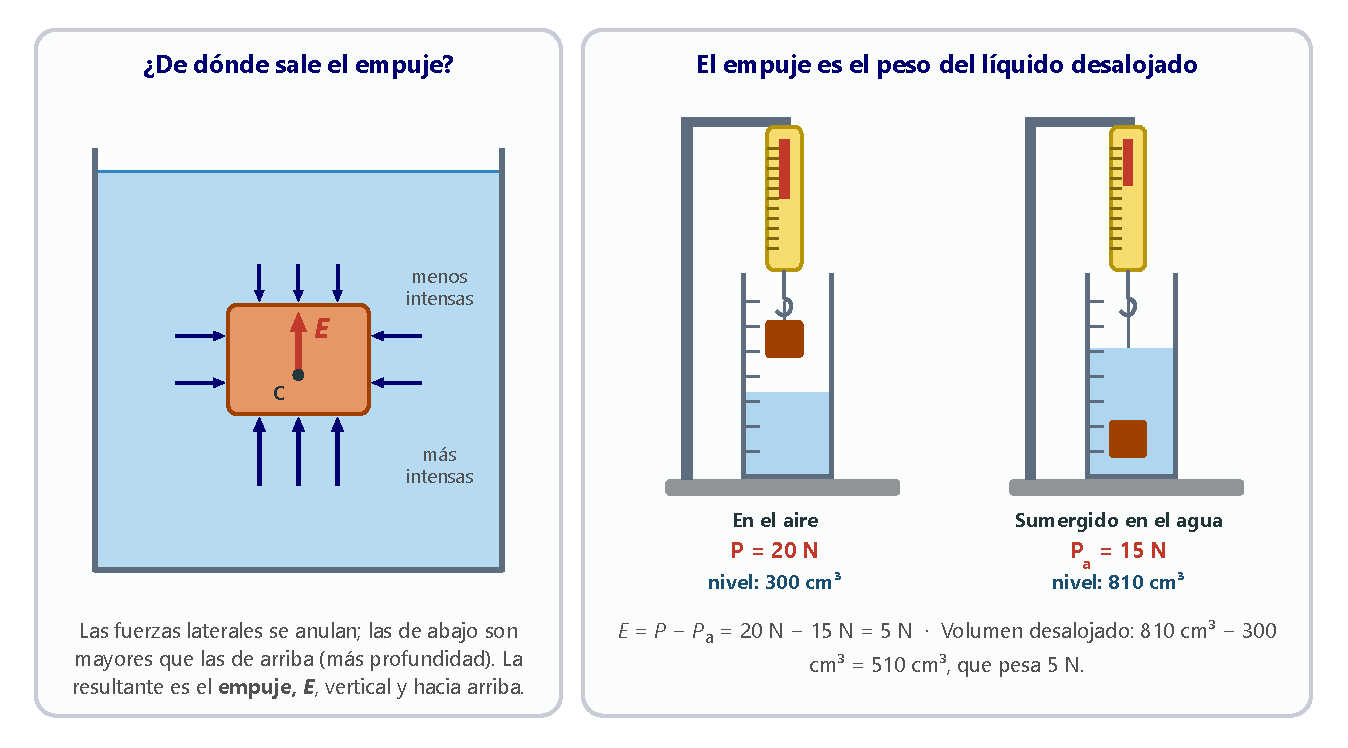
\includegraphics[width=\textwidth]{images/UD10/empuje}
    \caption{Origen de la fuerza de empuje y comprobación del principio de Arquímedes con un dinamómetro.}
    \label{fig:empuje}
\end{figure}

\subsection{¿Cómo se calcula el empuje? El peso aparente}

El empuje es el peso del fluido desalojado: \(E = m_{\text{fluido}} \cdot g\). Como \(m_{\text{fluido}} = \rho_{\text{fluido}} \cdot V_{\text{desalojado}}\), y el volumen desalojado es el volumen de la parte sumergida del cuerpo:
\[ E = V_{\text{sumergido}} \cdot \rho_{\text{fluido}} \cdot g \]

Se llama \textbf{peso aparente}, \(P_a\), al que marca el dinamómetro cuando el cuerpo está sumergido. Es el peso real menos el empuje:
\[ P_a = P - E \qquad\Rightarrow\qquad E = P - P_a \]
Si el cuerpo, de volumen \(V\), está totalmente sumergido, su peso es \(P = V \cdot \rho_{\text{cuerpo}} \cdot g\), y el peso aparente queda:
\[ P_a = V \cdot g \cdot (\rho_{\text{cuerpo}} - \rho_{\text{fluido}}) \]

El principio de Arquímedes es válido para todos los fluidos, líquidos y gases, y para cuerpos sumergidos total o parcialmente.

\begin{example}
    Una pieza de una aleación pesa \qty{400}{\newton} y ocupa \qty{5}{\cubic\dm}. Calcula el empuje que recibe al sumergirla en un líquido de densidad \qty{837}{\kg\per\cubic\m} y su peso aparente en él.
    \[ E = V \cdot \rho_{\text{líquido}} \cdot g = \num{5e-3} \cdot 837 \cdot \num{9.8} = \textcolor{red}{\qty{41}{\newton}} \qquad P_a = P - E = 400 - 41 = \textcolor{red}{\qty{359}{\newton}} \]
\end{example}

\subsection{¿Cómo se puede medir la densidad con el principio de Arquímedes?}

Muchos métodos para medir densidades se basan en este principio. Para un \textbf{sólido irregular}, basta con medir su peso en el aire, \(P\), y sumergido en agua, \(P_a\):
\begin{itemize}
    \item El empuje, \(E = P - P_a\), permite calcular el volumen: \(V = \dfrac{E}{\rho_{\text{agua}} \cdot g}\).
    \item El peso da la masa, \(m = P/g\), y la densidad es \(\rho = m/V\).
\end{itemize}
Combinando las dos expresiones se obtiene una fórmula muy cómoda: \(\rho_{\text{cuerpo}} = \rho_{\text{líquido}} \cdot \dfrac{P}{E}\).

Del mismo modo, si conocemos la densidad de un cuerpo, podemos medir la de un \textbf{líquido} pesando el cuerpo en el aire y sumergido en él. Los \textbf{densímetros} son tubos de vidrio lastrados que flotan en el líquido: cuanto más denso es, menos se hunden, y la densidad se lee en la escala, en la marca que coincide con la superficie.

\begin{example}
    Un objeto pesa \qty{300}{\newton} en el aire y \qty{200}{\newton} sumergido totalmente en agua. Calcula su volumen y su densidad.

    \(E = P - P_a = 300 - 200 = \qty{100}{\newton}\); \quad \(V = \dfrac{E}{\rho_{\text{agua}} \cdot g} = \dfrac{100}{1000 \cdot \num{9.8}} = \textcolor{red}{\qty{0.0102}{\cubic\m}}\).

    \(m = \dfrac{P}{g} = \dfrac{300}{\num{9.8}} = \qty{30.6}{\kg}\); \quad \(\rho = \dfrac{m}{V} = \dfrac{\num{30.6}}{\num{0.0102}} = \textcolor{red}{\qty{3000}{\kg\per\cubic\m}}\).

    Con la fórmula directa: \(\rho = 1000 \cdot \dfrac{300}{100} = \qty{3000}{\kg\per\cubic\m}\).
\end{example}

\begin{example}
    Una pieza de aluminio (\(\rho = \qty{2700}{\kg\per\cubic\m}\)) pesa \qty{350}{\newton} en el aire y \qty{230}{\newton} sumergida en un líquido. Calcula la densidad del líquido.

    \(E = 350 - 230 = \qty{120}{\newton}\). El volumen de la pieza es \(V = \dfrac{P}{\rho_{\text{Al}} \cdot g} = \dfrac{350}{2700 \cdot \num{9.8}} = \qty{0.01323}{\cubic\m}\), y por tanto:
    \[ \rho_{\text{líquido}} = \frac{E}{V \cdot g} = \frac{120}{\num{0.01323} \cdot \num{9.8}} = \textcolor{red}{\qty{926}{\kg\per\cubic\m}} \]
\end{example}

\subsection{¿Por qué flotan los cuerpos?}

Un cuerpo sumergido en un fluido está sometido a dos fuerzas: su \textbf{peso}, aplicado en su centro de gravedad, G, vertical y hacia abajo, y el \textbf{empuje}, aplicado en el centro de empuje, C, vertical y hacia arriba. Al soltarlo dentro del fluido puede ocurrir (figura~\ref{fig:flotacion}):
\begin{itemize}
    \item \(P > E\): el cuerpo \textbf{se hunde} hasta el fondo. Ocurre si \(\rho_{\text{cuerpo}} > \rho_{\text{fluido}}\); por ejemplo, una bola de hierro en agua.
    \item \(P = E\): el cuerpo queda \textbf{en equilibrio} dentro del fluido, sin subir ni bajar. Ocurre si \(\rho_{\text{cuerpo}} = \rho_{\text{fluido}}\); por ejemplo, un globo lleno de agua.
    \item \(P < E\): el cuerpo \textbf{sube y flota}. Ocurre si \(\rho_{\text{cuerpo}} < \rho_{\text{fluido}}\); por ejemplo, un corcho en agua. Al salir parcialmente, el volumen sumergido disminuye hasta que el empuje se iguala con el peso.
\end{itemize}

\begin{figure}[H]
    \centering
    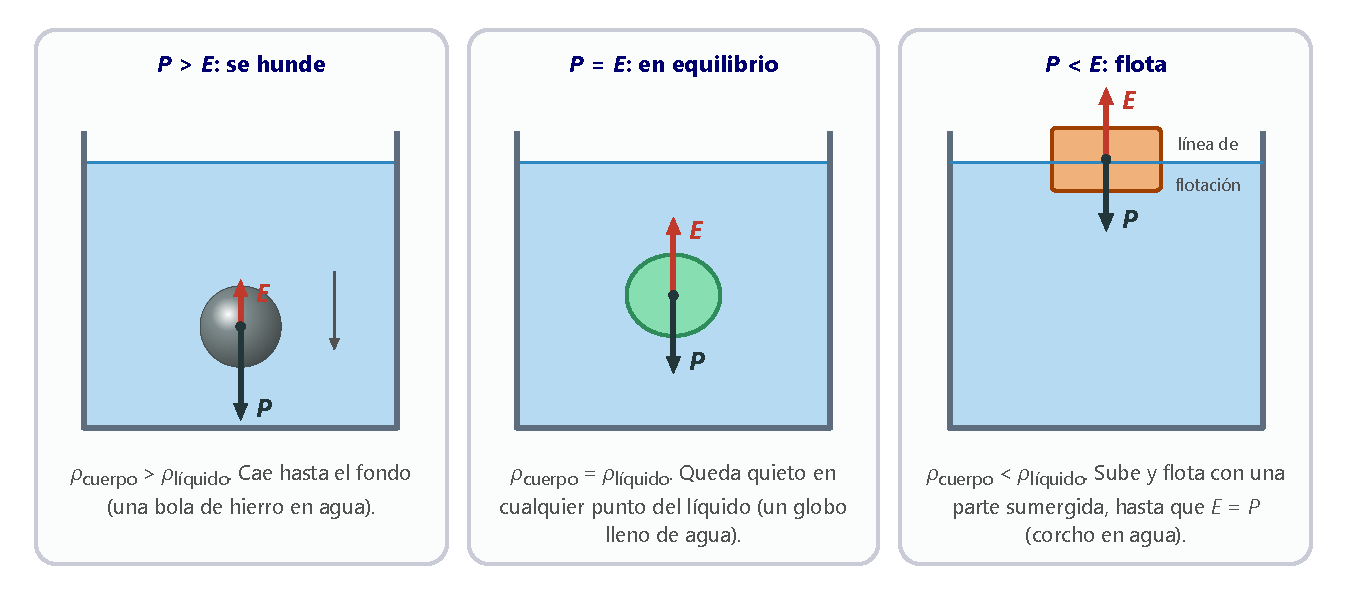
\includegraphics[width=\textwidth]{images/UD10/flotacion}
    \caption{Un cuerpo se hunde, queda en equilibrio o flota según sean su peso y el empuje.}
    \label{fig:flotacion}
\end{figure}

Para un cuerpo que flota, \(E = P\), es decir, \(V_{\text{sumergido}} \cdot \rho_{\text{fluido}} \cdot g = V \cdot \rho_{\text{cuerpo}} \cdot g\), de donde:
\[ \frac{V_{\text{sumergido}}}{V} = \frac{\rho_{\text{cuerpo}}}{\rho_{\text{fluido}}} \]

\begin{example}
    ¿Qué fracción de un iceberg queda bajo el agua? (\(\rho_{\text{hielo}} = \qty{917}{\kg\per\cubic\m}\); \(\rho_{\text{agua de mar}} = \qty{1030}{\kg\per\cubic\m}\)).
    \[ \frac{V_{\text{sumergido}}}{V} = \frac{917}{1030} = \num{0.89} \]
    El \textcolor{red}{\qty{89}{\percent}} del iceberg está sumergido: solo vemos la «punta del iceberg».
\end{example}

\paragraph{¿Por qué flota un barco de acero?} El acero es casi ocho veces más denso que el agua, pero un barco es hueco: su volumen total es enorme y su densidad \emph{media} (acero, aire y carga) es menor que la del agua. Al hundirse un poco desaloja mucha agua, y el empuje compensa su peso. La línea que separa la parte sumergida del casco de la que no lo está es la \textbf{línea de flotación}; si aumenta la carga, el barco se hunde más hasta que el empuje vuelve a igualar al peso.

Para que un barco esté en equilibrio estable, además de ser \(P = E\), el centro de gravedad y el centro de empuje deben estar en la misma vertical, y \textbf{G debe estar más bajo que C} (figura~\ref{fig:barco_globo}). Así, si una ola lo inclina, el par de fuerzas formado por el peso y el empuje lo vuelve a poner derecho. Por eso la carga pesada se coloca lo más abajo posible.

\paragraph{¿Por qué sube un globo aerostático?} El principio de Arquímedes también se cumple en el aire. Un globo se llena de aire caliente (o de helio), menos denso que el aire que lo rodea; como su volumen es muy grande, el empuje del aire es mayor que el peso total del globo, y sube.

\begin{figure}[H]
    \centering
    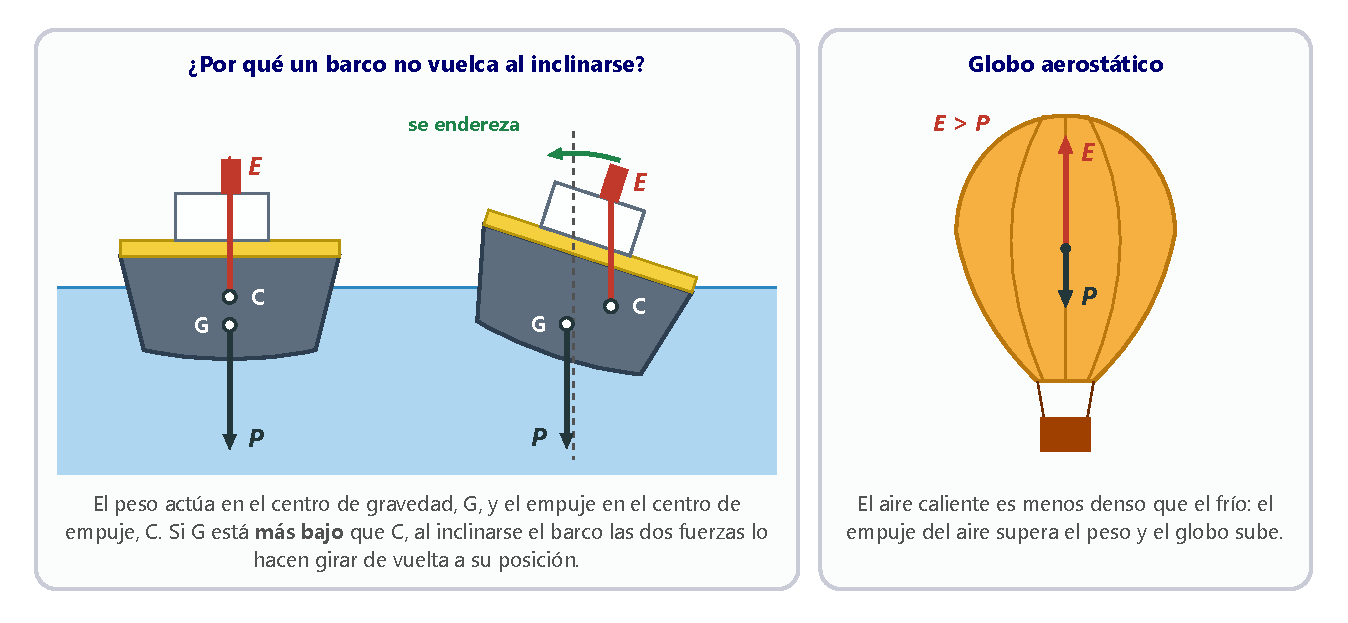
\includegraphics[width=\textwidth]{images/UD10/barco_globo}
    \caption{Estabilidad de un barco y flotación de un globo aerostático.}
    \label{fig:barco_globo}
\end{figure}

\begin{exercise}
    Una piedra pesa \qty{300}{\newton} en el aire y \qty{280}{\newton} sumergida en agua. ¿Cuál es su volumen?
    \begin{solu}
        \(E = P - P_a = 300 - 280 = \qty{20}{\newton}\); \(V = \dfrac{E}{\rho_{\text{agua}} \cdot g} = \dfrac{20}{1000 \cdot \num{9.8}} = \textcolor{red}{\qty{2.04e-3}{\cubic\m}} = \qty{2.04}{\cubic\dm}\).
    \end{solu}
\end{exercise}

\begin{exercise}
    Se sumerge en agua un cuerpo de \qty{300}{\gram} y \qty{20}{\cubic\cm}. ¿Cuál es su peso? ¿Qué empuje recibe? ¿Cuál es su peso aparente?
    \begin{solu}
        \(P = \num{0.300} \cdot \num{9.8} = \textcolor{red}{\qty{2.94}{\newton}}\); \quad \(E = \num{2e-5} \cdot 1000 \cdot \num{9.8} = \textcolor{red}{\qty{0.196}{\newton}}\); \quad \(P_a = \num{2.94} - \num{0.196} = \textcolor{red}{\qty{2.74}{\newton}}\).
    \end{solu}
\end{exercise}

\begin{exercise}
    Busca información sobre cómo se usa en el laboratorio un densímetro para medir la densidad de un líquido. ¿Por qué se hunde más en el alcohol que en el agua?
    \begin{solu}
        Respuesta libre. Se introduce el densímetro en una probeta con el líquido, se deja que flote libremente y se lee la marca de la escala que coincide con la superficie del líquido. En el alcohol, que es \textcolor{red}{menos denso}, el densímetro tiene que \textcolor{red}{desalojar más volumen} para que el empuje iguale a su peso, y por eso se hunde más.
    \end{solu}
\end{exercise}

\begin{exercise}
    Una esfera pesa \qty{176}{\newton} en el aire y \qty{126}{\newton} sumergida totalmente en agua. Calcula su volumen y su densidad.
    \begin{solu}
        \(E = 176 - 126 = \qty{50}{\newton}\); \(V = \dfrac{50}{1000 \cdot \num{9.8}} = \textcolor{red}{\qty{5.1e-3}{\cubic\m}}\).
        \(\rho = \rho_{\text{agua}} \cdot \dfrac{P}{E} = 1000 \cdot \dfrac{176}{50} = \textcolor{red}{\qty{3520}{\kg\per\cubic\m}}\).
    \end{solu}
\end{exercise}

\begin{exercise}
    Una pieza de plata (\(\rho = \qty{10500}{\kg\per\cubic\m}\)) pesa \qty{500}{\newton} en el aire y \qty{420}{\newton} sumergida en un líquido. Calcula la densidad del líquido.
    \begin{solu}
        \(E = 500 - 420 = \qty{80}{\newton}\); \(V = \dfrac{P}{\rho_{\text{plata}} \cdot g} = \dfrac{500}{10500 \cdot \num{9.8}} = \qty{4.86e-3}{\cubic\m}\).
        \(\rho_{\text{líquido}} = \dfrac{E}{V \cdot g} = \dfrac{80}{\num{4.86e-3} \cdot \num{9.8}} = \textcolor{red}{\qty{1680}{\kg\per\cubic\m}}\).
    \end{solu}
\end{exercise}

\begin{exercise}
    ¿Qué hace un submarino para sumergirse y para volver a la superficie?
    \begin{solu}
        Cambia su \textcolor{red}{peso} sin cambiar su volumen (y, por tanto, su empuje): para sumergirse \textcolor{red}{llena de agua} unos depósitos (tanques de lastre) y para subir los \textcolor{red}{vacía} expulsando el agua con aire comprimido.
    \end{solu}
\end{exercise}

\begin{exercise}
    ¿Cómo cambia la línea de flotación de un barco cuando pasa de un río al mar? ¿Por qué?
    \begin{solu}
        El agua del mar es \textcolor{red}{más densa} que la del río. Para conseguir el mismo empuje (igual al peso del barco) necesita desalojar menos volumen, así que en el mar el barco \textcolor{red}{se hunde menos}: la línea de flotación queda más alta respecto al agua.
    \end{solu}
\end{exercise}

\subsection*{Actividades de consolidación: empuje y principio de Arquímedes}

\begin{exercise}
    Justifica si son verdaderas o falsas estas afirmaciones:
    \begin{enumerate}[label=\alph*)]
        \item La línea de acción del empuje pasa siempre por el centro de gravedad del cuerpo sumergido.
        \item Dos cuerpos distintos del mismo volumen, totalmente sumergidos en el mismo líquido, reciben el mismo empuje.
        \item El empuje es igual a la diferencia entre el peso del cuerpo en el aire y su peso aparente en el líquido.
        \item El empuje es proporcional al volumen de líquido desalojado, a la gravedad y a la densidad del líquido.
    \end{enumerate}
    \begin{solu}
        a) \textcolor{red}{Falso}: pasa por el \emph{centro de empuje}, que es el centro de gravedad del fluido desalojado. Solo coincide con el centro de gravedad del cuerpo si este es homogéneo y está totalmente sumergido (en un barco, por ejemplo, no coinciden).
        b) \textcolor{red}{Verdadero}: el empuje depende del volumen desalojado, no del material. c) \textcolor{red}{Verdadero}. d) \textcolor{red}{Verdadero}: \(E = V \cdot \rho \cdot g\).
    \end{solu}
\end{exercise}

\begin{exercise}
    Explica qué ocurre en cada caso y qué conclusión general se obtiene:
    \begin{enumerate}[label=\Alph*)]
        \item Un globo de aire caliente en el aire frío.
        \item Un bloque de densidad \qty{300}{\kg\per\cubic\m} en agua.
        \item Un bloque de densidad \qty{790}{\kg\per\cubic\m} en agua.
        \item Un bloque de densidad \qty{790}{\kg\per\cubic\m} en alcohol (\qty{790}{\kg\per\cubic\m}).
        \item Un bloque de plomo (\qty{11300}{\kg\per\cubic\m}) en agua.
    \end{enumerate}
    \begin{solu}
        A) El aire caliente es menos denso que el frío: el globo \textcolor{red}{sube}.
        B) Flota con solo el \qty{30}{\percent} de su volumen sumergido.
        C) También \textcolor{red}{flota}, pero más hundido que B: el \qty{79}{\percent} de su volumen está sumergido.
        D) Las densidades son iguales: queda \textcolor{red}{en equilibrio} en cualquier punto del líquido.
        E) Es mucho más denso que el agua: \textcolor{red}{se hunde}.
        Conclusión: un cuerpo \textcolor{red}{flota} si es menos denso que el fluido, queda \textcolor{red}{en equilibrio} si tiene su misma densidad y \textcolor{red}{se hunde} si es más denso.
    \end{solu}
\end{exercise}

\begin{exercise}
    Queremos saber si una joya es de oro puro (\(\rho = \qty{19300}{\kg\per\cubic\m}\)). Su masa es de \qty{0.120}{\kg} y, sumergida en agua, su peso aparente equivale al de una masa \qty{8}{\gram} menor. ¿Es de oro puro?
    \begin{solu}
        El empuje equivale al peso de \qty{8}{\gram} de agua, que ocupan \qty{8}{\cubic\cm}: \(V_{\text{joya}} = \qty{8e-6}{\cubic\m}\).
        \(\rho = \dfrac{\num{0.120}}{\num{8e-6}} = \qty{15000}{\kg\per\cubic\m}\). Es menor que la del oro: \textcolor{red}{no es de oro puro}.
    \end{solu}
\end{exercise}

\begin{exercise}
    Un objeto de \qty{10000}{\newton} de peso ocupa \qty{10}{\cubic\m}. ¿Flotará en un tanque lleno de aceite de densidad \qty{935}{\kg\per\cubic\m}? ¿Qué fracción de su volumen quedará sumergida?
    \begin{solu}
        \(m = \dfrac{10000}{\num{9.8}} = \qty{1020}{\kg}\); \(\rho = \dfrac{1020}{10} = \qty{102}{\kg\per\cubic\m}\). Es menos denso que el aceite: \textcolor{red}{sí flota}.
        Fracción sumergida: \(\dfrac{102}{935} = \num{0.11}\), es decir, el \textcolor{red}{\qty{11}{\percent}}.
    \end{solu}
\end{exercise}

\begin{exercise}
    Un cubo de madera de \qty{10}{\cm} de arista flota en agua con \qty{6}{\cm} sumergidos. ¿Cuál es la densidad de la madera? ¿Cuántos centímetros se hundiría en aceite de densidad \qty{800}{\kg\per\cubic\m}?
    \begin{solu}
        \(\dfrac{\rho_{\text{madera}}}{\rho_{\text{agua}}} = \dfrac{V_{\text{sumergido}}}{V} = \dfrac{6}{10} \Rightarrow \rho_{\text{madera}} = \textcolor{red}{\qty{600}{\kg\per\cubic\m}}\).
        En aceite: \(\dfrac{h}{10} = \dfrac{600}{800} = \num{0.75} \Rightarrow h = \textcolor{red}{\qty{7.5}{\cm}}\).
    \end{solu}
\end{exercise}
